\documentclass[11pt, a4paper]{article}

% --- ESSENTIAL PACKAGES ---

% Font Encoding and Input
\usepackage[T1]{fontenc} % Use 8-bit T1 fonts to ensure proper character rendering
\usepackage[utf8]{inputenc} % Allows direct use of UTF-8 characters (e.g., é, ö, à)
\usepackage{amsmath} % For \text{} in math mode

% Page Layout and Margins
\usepackage{geometry}
\geometry{
    a4paper,
    left=1.5cm,
    right=1.5cm,
    top=2.5cm,
    bottom=1.5cm
}
\usepackage{setspace}
\usepackage{etoolbox}
\usepackage[english, bidi=basic, provide=*]{babel}
\babelprovide[import, onchar=ids fonts]{english}

\usepackage{enumitem}
\setlist[itemize]{label=-}
% --- END UNIVERSAL PREAMBLE BLOCK ---

\usepackage{booktabs}   % For professional-looking rules (\toprule, \midrule, \bottomrule)
\usepackage{longtable}  % The package that allows tables to break across pages
\usepackage{lipsum}     % For generating dummy text to show the page break

% --- FIXED PACKAGE LOADING ---
% Removed trailing non-breaking spaces after package names, which were causing the error.
\usepackage{array}    % For defining column types
\usepackage{ragged2e} % For RaggedRight alignment
\usepackage{amsmath}  % Required for math symbols like \ge and \le
\usepackage{cite}     % To handle citations
% --- END FIX ---
% Professional Fonts (Times New Roman)
\usepackage{times}
% \usepackage{helvet} % For Helvetica font, used for the main title
\usepackage{fancyhdr}

% --- FANCY HEADER CONFIGURATION ---
% \fancyhf{} % Clear all default header and footer fields
% \lhead{\footnotesize Call: [insert call identifier] — [insert call name]}
% \rhead{\footnotesize EU Grants: Application form (HE EIC Pathfinder Challenges): V3.4 – 12.06.2024}
% \cfoot{\footnotesize \thepage} % Use \small for the footer too for consistency
% \renewcommand{\headrulewidth}{0.4pt} % Adds a thin line under the header


% --- FANCY HEADER CONFIGURATION (TWO-LINE, SPLIT ALIGNMENT) ---
\fancyhf{} % Clear all default header and footer fields

% We put everything in \lhead and use a tabular* to span the page
% and control the left/right alignment of each line.
\lhead{%
  \begin{tabular*}{\textwidth}{@{} l r @{}} % Spans text width, no padding
    \footnotesize Call: [insert call identifier] — Generative-AI based Agents to Revolutionize Medical Diagnosis and Treatment of Cancer & \\ % Line 1, left
    \footnotesize EU Grants: Application form (HE EIC Pathfinder Challenges): V3.4 – 12.06.2024 % Line 2, right
  \end{tabular*}%
}

\cfoot{\footnotesize \thepage} % Adds the page number (footnotesize)
\renewcommand{\headrulewidth}{0.4pt} % Adds a thin line under the header
% --- END HEADER CONFIGURATION ---
% --- END HEADER CONFIGURATION ---


% --- BIBLIOGRAPHY (using biblatex) ---
\usepackage[
    backend=biber,
    style=numeric-comp,
    sorting=none,
    maxbibnames=0,
    minbibnames=0,
    % --- MODIFIED FOR DOI ONLY ---
    doi=true,         % Print DOI
    url=false,        % Don't print URL
    isbn=false,       % Don't print ISBN
    eprint=false      % Don't print eprint (like arXiv)
]{biblatex}

% --- Add AFTER \usepackage{biblatex} ---
\AtEveryBibitem{%
  \clearfield{author}%
  \clearfield{title}%
  \clearfield{journaltitle}%
}
% --- TIGHTER SPACING OPTIONS ---

% 1. Set vertical space BETWEEN items to zero
\setlength{\bibitemsep}{0pt} 

% 2. (Optional) Remove "In:" for articles/books
% \renewbibmacro{in:}{}

% 3. (Optional) Remove "pp." or "pages"
% \DeclareFieldFormat{pages}{#1}

% --- END COMPACT OPTIONS ---

% Load your .bib file
\addbibresource{bibl.bib} 
% --- END BIBLIOGRAPHY ---

% Color Management
\usepackage[dvipsnames]{xcolor} % Use dvipsnames for a wider range of predefined colors

% Define a professional color palette
\definecolor{primary}{HTML}{0A369D}  % A deep, professional blue
\definecolor{secondary}{HTML}{4472CA} % A lighter, complementary blue
\definecolor{darkgray}{HTML}{333333}  % For body text, better than pure black
\definecolor{customgreen}{HTML}{5E8B7E} % A muted green for accents
\definecolor{titleblue}{HTML}{082A75} % A darker, rich blue for the main title

\color{darkgray} % Set the default text color

% Section and Title Styling
\usepackage{titlesec}
\titleformat{\section}
  {\normalfont\Large\bfseries\color{primary}} % Format for the section title
  {\thesection}{1em}{} % Section number, spacing, and the title itself
\titleformat{\subsection}
  {\normalfont\large\bfseries\color{secondary}}
  {\thesubsection}{1em}{}
\titleformat{\subsubsection}
  {\normalfont\bfseries\color{customgreen}}
  {\thesubsubsection}{1em}{}

% --- IMAGES AND GRAPHICS ---

% Standard package for including images
\usepackage{graphicx}
\graphicspath{{images/}} % Optional: specify a folder for your images
\usepackage{float} % Improved control over figure placement with [H] option

% --- LISTS AND ENUMERATIONS ---

% Customize list environments
\usepackage{enumitem}
% The 'textcolor' option sets the color for the item's text
\setlist[itemize,1]{label=\textcolor{primary}{\textbullet}}
\setlist[itemize,2]{label=\textcolor{secondary}{\textendash}}

% --- HYPERLINKS ---

% Hyperlink styling for URLs and cross-references
\usepackage{hyperref}
\hypersetup{
    colorlinks=true,
    linkcolor=primary,
    filecolor=magenta,
    urlcolor=secondary,
    citecolor=customgreen,
    pdftitle={My Professional Document},
    pdfpagemode=FullScreen,
}



% --- UNIVERSAL PREAMBLE BLOCK (PDFLATEX COMPATIBLE) ---
\usepackage[a4paper, top=2.5cm, bottom=2.5cm, left=2cm, right=2cm]{geometry}

\usepackage[utf8]{inputenc} % Allows UTF-8 input
\usepackage[T1]{fontenc}    % Use 8-bit T1 fonts
\usepackage[english]{babel}   % Standard babel for English
% --- END FONT/ENCODING FIX ---

\usepackage{enumitem} % For list formatting
\setlist[itemize]{label=-}
% --- END UNIVERSAL PREAMBLE BLOCK ---

\usepackage{booktabs} % For professional looking rules in tables
\usepackage{longtable} % For tables that span multiple pages

% --- FIXED PACKAGE LOADING ---
\usepackage{array}    % For defining column types
\usepackage{ragged2e} % For RaggedRight alignment
\usepackage{amsmath}  % Required for math symbols like \ge and \le
\usepackage{cite}     % To handle citations
% --- END FIX ---

% Define column types for text wrapping
\newcolumntype{L}[1]{>{\RaggedRight\arraybackslash}p{#1}}



% --- TYPOGRAPHY AND MICRO-ADJUSTMENTS ---

% Improves the justification and spacing of text for a cleaner look
\usepackage{microtype}

% --- DOCUMENT CONTENT EXAMPLE ---

% For placeholder text
\usepackage{lipsum}

% --- TABLE AND CURRENCY PACKAGES ---
\usepackage{booktabs} % For professional looking tables
\usepackage{longtable} % For tables that may span multiple pages
\usepackage{siunitx} % For aligning numbers in tables
\usepackage{eurosym} % For the EUR symbol
\usepackage{float} % to use [H]
\usepackage{ragged2e}
\usepackage{pdfpages}

% --- GLOSSARIES ---
\usepackage[acronym]{glossaries}
\makeglossaries

\newacronym{genai}{GenAI}{Generative AI}
\newacronym{pca}{PCa}{Prostate Cancer}
\newacronym{njde}{NJDE}{Neural Jump Ordinary Differential Equation}
\newacronym{mri}{MRI}{Magnetic Resonance Imaging}
\newacronym{pet}{PET}{Positron Emission Tomography}
\newacronym{ct}{CT}{Computed Tomography}
\newacronym{ehr}{EHR}{Electronic Health Record}
\newacronym{vae}{VAE}{Variational Autoencoder}
\newacronym{trl}{TRL}{Technology Readiness Level}
\newacronym{psma}{PSMA}{Prostate-Specific Membrane Antigen}
\newacronym{ttp}{TTP}{Time-to-Progression}
\newacronym{eau}{EAU}{European Association of Urology}
\newacronym{wsi}{WSI}{Whole-Slide Images}
\newacronym{tcga}{TCGA-PRAD}{The Cancer Genome Atlas - Prostate Adenocarcinoma}
\newacronym{eucaim}{EUCAIM}{European Cancer Imaging Initiative}
\newacronym{sla}{SLA}{Service Level Agreement}
\newacronym{cdm}{CDM}{Common Data Model}
\newacronym{omopcdm}{OMOP-CDM}{Observational Medical Outcomes Partnership - Common Data Model}
\newacronym{fhir}{HL7 FHIR}{Health Level Seven - Fast Healthcare Interoperability Resources}
\newacronym{dsa}{DSA}{Data Sharing Agreement}
\newacronym{gdpr}{GDPR}{General Data Protection Regulation}
\newacronym{fid}{FID}{Fréchet Inception Distance}
\newacronym{ssim}{SSIM}{Structural Similarity Index Measure}
\newacronym{lpips}{LPIPS}{Learned Perceptual Image Patch Similarity}
\newacronym{auc}{AUC}{Area Under the Curve}
\newacronym{mae}{MAE}{Mean Absolute Error}
\newacronym{cindex}{C-index}{Concordance Index}
\newacronym{ood}{OOD}{Out-of-Distribution}
\newacronym{xai}{XAI}{eXplainable AI}
\newacronym{eibir}{EIBIR}{European Institute for Biomedical Imaging Research}
\newacronym{dicom}{DICOM}{Digital Imaging and Communications in Medicine}
\newacronym{adt}{ADT}{Androgen Deprivation Therapy}
\newacronym{ap}{AP}{Alkaline Phosphatase}
\newacronym{asap}{ASAP}{Atypical Small Acinar Proliferation}
\newacronym{bcr}{BCR}{Biochemical Recurrence}
\newacronym{bph}{BPH}{Benign Prostatic Hyperplasia}
\newacronym{crpc}{CRPC}{Castration-Resistant Prostate Cancer}
\newacronym{ctc}{CTCs}{Circulating Tumor Cells}
\newacronym{ece}{ECE}{Extracapsular Extension}
\newacronym{ene}{ENE}{Extranodal Extension}
\newacronym{hgpin}{HGPIN}{High-Grade Prostatic Intraepithelial Neoplasia}
\newacronym{lvi}{LVI}{Lymphovascular Invasion}
\newacronym{psadt}{PSADT}{PSA Doubling Time}



\begin{document}

\pagestyle{fancy}
\thispagestyle{fancy}

\title{A Causal AI Framework for Longitudinal Modelling of Prostate Cancer}

% 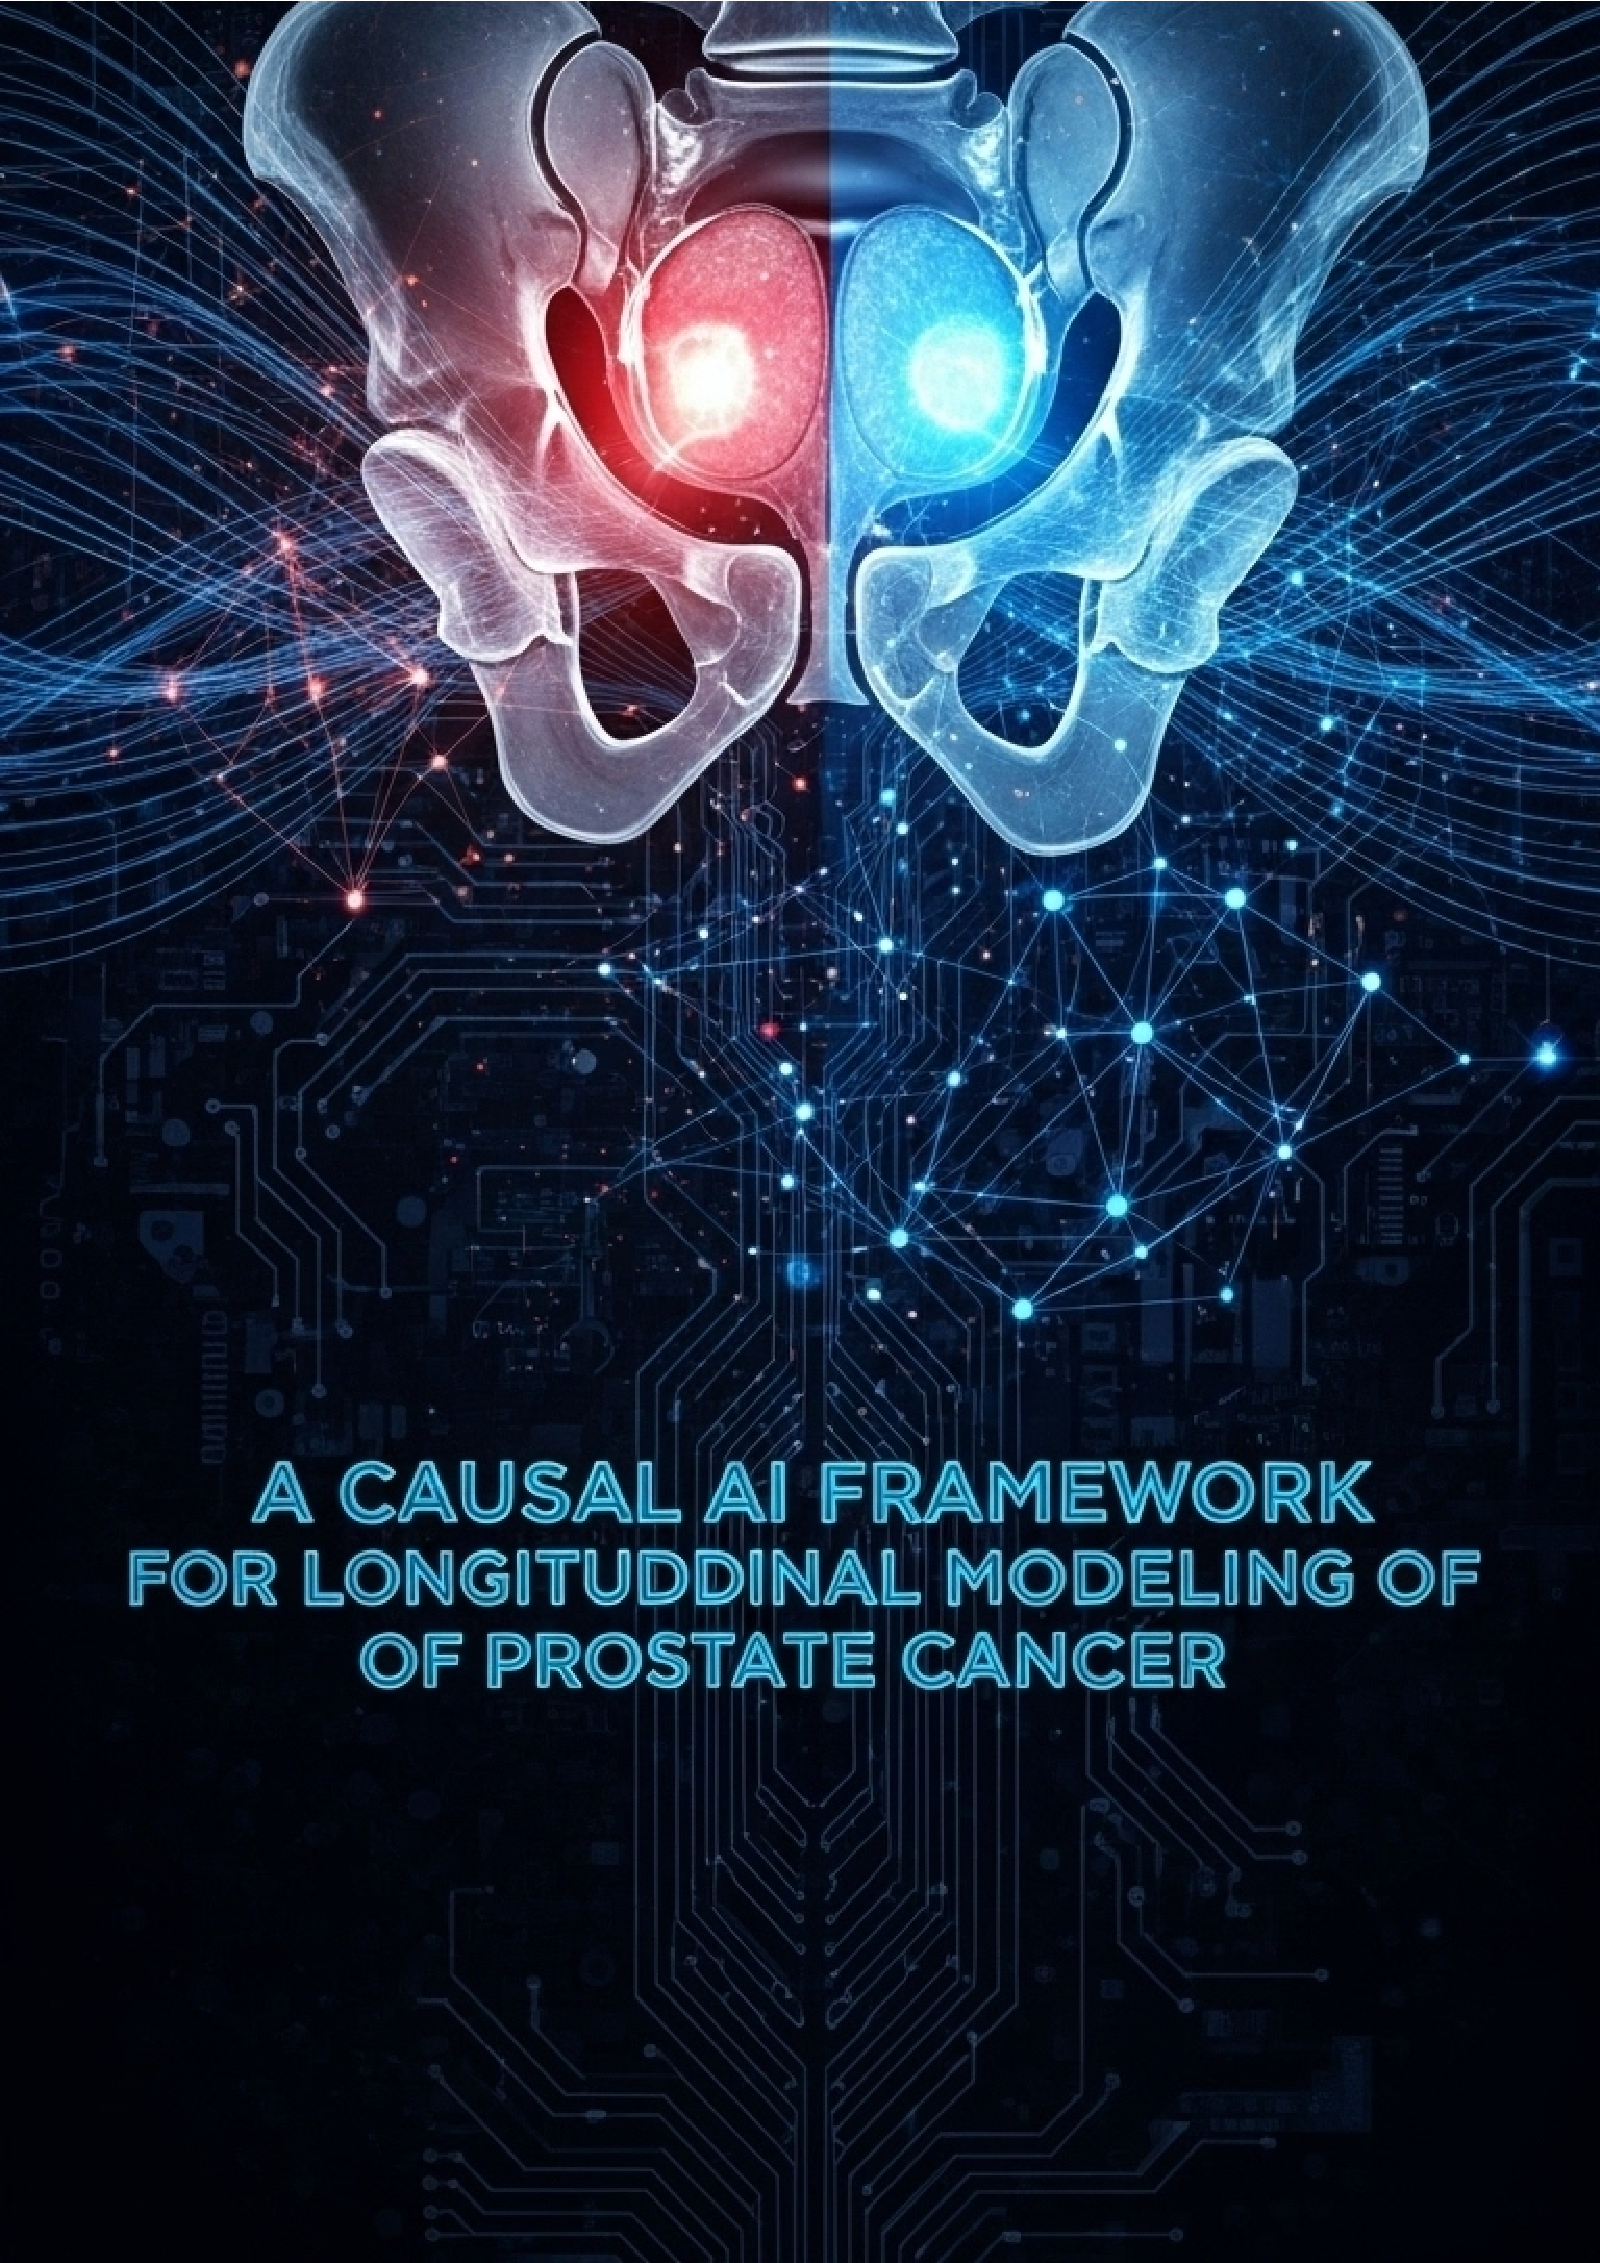
\includepdf[pages=-]{title_page.pdf}

\begin{figure}[H]
    \centering
    
\includegraphics[        trim=35mm 18mm 35mm 18mm, % {left bottom right top}
        clip,                     % This command applies the trim
        width=0.9\textwidth]{graphical_abstract.png}
    \caption{Graphical abstract}
    \label{fig:graphical_abstract}
\end{figure}


\maketitle
\thispagestyle{fancy}

% \begin{abstract}
% This project introduces a new paradigm in oncology with an interactive, Generative AI (GenAI)-based agent for managing prostate cancer (PCa) at any stage of the disease. We focus on prostate cancer and address both clinical objectives - predictive diagnosis and personalized treatment selection - while advancing all three technological objectives: multimodal integration, medical data augmentation, and knowledge representation. We will build a causal "digital twin" to transparently model the disease trajectory by integrating complex multimodal data into a unified, personalized patient view. Technologically, we will fuse multimodal data from internal and external sources, use GenAI for data augmentation, and infuse deep medical domain knowledge like local and international guidelines into the novel model's architecture to guide its learning process and disentangle disease signals from confounders. This should be a solid basis for generating the synthesized data for further experiments. Clinically, our agent will improve diagnostic interpretation by simulating disease progression and enable personalized treatment selection by forecasting outcomes. The framework is designed as a trustworthy, explainable, and safe AI system compliant with the EU AI Act, establishing a new European standard for medical GenAI. 
% \end{abstract}



\section{Excellence}

\subsection{Objectives and Relevance to the Challenge}
Our proposal addresses both the technological and clinical areas of the call. Building on the identified challenges of disease heterogeneity, therapy-driven evolution, and diagnostic uncertainty, our approach aims to resolve these unmet needs through a new generation of causal, explainable GenAI agents that model disease dynamics and guide therapy adaptation. We will build interactive autonomous agents, composable into a super-agent, that deliver an end-to-end, clinician-in-the-loop pathway from risk assessment to therapy selection and follow-up (As shown in Figure \ref{fig:graphical_abstract}) .  At its core is a causal digital twin that fuses longitudinal, multidimensional, and multimodal evidence (MRI/CT/PET, pathology, hospital records, data from local and state cancer registries, labs, genomics, and expert knowledge incl. medical guideliness) into a unified, actionable patient state. The models perform predictive diagnosis and personalised treatment selection, with calibrated uncertainty, interpretable rationales, and clinician-facing explanations. To overcome data scarcity and bias, we will generate and share high-fidelity synthetic data and contribute to a representative, reliable common database across the portfolio. Compliance with the EU concept of Trustworthy AI, the AI Act and MDR is embedded by design, alongside robust security, privacy and auditability. 
We will validate the (super-)agent using diverse multi-centre datasets and harmonised protocols and by running pre-registered controlled proof-of-concept studies covering both inpatient and outpatient care. We will also open our clinical platform for external validation of complementary and/or alternative concepts. The result we want to achieve is a scalable European benchmark for safe, effective, and sustainable AI that reduces diagnostic variability, personalises care, and lightens clinician workload. 
 
\subsubsection*{Area 1: Technological Area}
\begin{itemize}
 
    \item \textbf{Advanced Medical Dataset Synthesis via \gls{genai} (ii):} Our framework will leverage advanced \gls{genai} techniques to create new, high-fidelity synthetic medical datasets. This synthesis will be achieved through two primary methods. Firstly, we will generate \textbf{counterfactual images} that introduce controlled variations, such as synthesizing a patient's scan at a different age or disease stage to isolate the visual impact of these factors. Secondly, we will perform \textbf{cross-modality synthesis} (e.g., generating a synthetic \gls{ct} from an existing \gls{mri}) with the specific aim of creating complete data pairs. This comprehensive approach to data synthesis directly tackles the common clinical problem of missing modalities. The resulting synthetic datasets will then be used to enable robust data augmentation, facilitate more effective multi-modal model training and fusion, and accelerate research and development across the EIC portfolio.
    
    \item \textbf{\gls{genai}-based tools for Integrating Multidimensional Multimodal Health Data (i):} We will develop and validate a novel Causal AI framework, built upon a \gls{njde} architecture. This model will pioneer the integration of multicenter (see table \ref{tab:data}  ), multidimensional and multimodal data—including imaging (\gls{mri}, \gls{pet}, \gls{ct}), \gls{ehr}, pathology, and -omics data—into a unified, dynamic patient model. This foundational technology will establish a reference architecture for trustworthy, causal medical AI. The successful development of this framework will be validated by milestones M3 and M4, which assess the core components of VAE-based disentanglement and temporal trajectory modeling. A key technical objective is to master data heterogeneity through a robust \gls{vae} framework that disentangles true disease signals from confounders, ensuring the model is robust and generalizable across diverse European healthcare systems.



    \item \textbf{Medical Knowledge Integration via Strong Inductive Biases (iii):} Our framework moves beyond simplistic "black-box" models by creating a comprehensive medical knowledge base, not as a separate component, but by deeply embedding extensive domain knowledge directly into the model's architecture and training process. This is achieved through a multi-layered strategy of applying strong, clinically-informed inductive biases:
    \begin{itemize}
        \item \textbf{At the Feature Level:} We will incorporate prognostic features explicitly recommended by urological guidelines \cite{guidelines_uro_1,guidelines_uro_2} , such as \gls{psadt} and tumor volume, directly into the model's input, ensuring it is grounded in established clinical practice.
        \item \textbf{At the Architectural Level:} The core of our knowledge integration lies in the principled disentanglement of the \gls{vae}'s latent space. This approach mirrors the clinical reasoning process where physicians mentally separate the \textbf{disease state} (e.g., TNM stage) from the overall \textbf{patient state} (e.g., age, frailty, comorbidities) before fusing the information. Our model operationalizes this by architecturally separating these factors into distinct latent subspaces. Furthermore, this technique is used to explicitly disentangle and isolate known technical \textbf{confounders}, such as differences in scanner type or imaging protocol, ensuring the learned disease representation is robust to these variations.
        \item \textbf{At the Objective Level:} We will use specialized, knowledge-infused loss functions. For ordinal variables like Gleason Grade or PI-RADS scores, a \textbf{differential ordinal loss} ensures the model understands their inherent ranking and severity progression, a concept a standard classification loss ignores.
        \item \textbf{At the Training Strategy Level:} The temporal model (\gls{njde}) will be pre-trained on a simplified, rule-based decision algorithm derived directly from established \textbf{\gls{eau} clinical guidelines} \cite{guidelines_uro_1,guidelines_uro_2}. This provides the model with a robust, clinically-valid starting point for understanding disease progression before fine-tuning on complex real-world data.
    \end{itemize}
    This multi-faceted infusion of domain knowledge ensures the model learns the true underlying causal mechanisms of the disease. The resulting clinically plausible, visual counterfactuals are a direct output of this knowledge-grounded architecture, enabling clinicians to ask meaningful "what-if" questions and receive intuitive, reliable explanations. Robust methods for uncertainty quantification will also be integrated to reliably flag high-uncertainty cases for human review. The effectiveness of this deep knowledge integration will be rigorously proven through a series of ablation studies, as detailed in our validation strategy.
\end{itemize}

\subsubsection*{Area 2: Clinical Area}
We propose to focus primarily on the early and progressive stages of cancer development (from Gleason 6 and active surveillance to palliative therapy), reflecting our team’s specific expertise. We will also share our data with other selected projects from the portfolio that focus on predictive diagnosis to jointly identify characteristic features of this subgroup of patients compared to the rest of the population, as well as potential correlations and causal relationships. 
\begin{itemize}
    \item \textbf{Predictive Diagnosis  (i):} We will develop an interactive agent capable of providing a personalized, dynamic prognosis. The agent will simulate a patient's future disease trajectory, generating predictions of not only future scans but also key, validated clinical endpoints such as future \textbf{TNM stage, PI-RADS scores}, and the likelihood of \textbf{\gls{bcr}}. The achievement of this objective will be directly verified by Milestone M4, which sets a clear performance target for the prediction of these key clinical endpoints. This provides a comprehensive prognostic tool to improve diagnostic precision and risk stratification, reducing over- and under-treatment. Furthermore, this simulation capability transforms the model into a powerful platform for \textit{in-silico} clinical trials. By modeling counterfactual patient journeys under different diagnostic or therapeutic assumptions, we can generate and pre-test robust research hypotheses, allowing for the design of more targeted and efficient human clinical trials in the future.

    \item \textbf{Enhance Personalized Treatment Selection (ii):} We will deliver a treatment-choice helper that, while respecting the \textbf{\gls{eau} guidelines} as the gold standard, directly addresses their acknowledged evidence gaps. The agent will leverage the "digital twin" to forecast outcomes for different treatment pathways, optimizing for maximum \gls{ttp}. The utility of this treatment-choice helper will be confirmed in Milestone M5, where its outputs will be validated by clinical experts for plausibility and usefulness. Critically, this will help resolve uncertainty around the use of \textbf{\gls{psma} \gls{pet}/\gls{ct}}. While its high sensitivity for early disease detection is known, a lack of extensive clinical trial data means guidelines cannot yet specify how to best act on this information. Our model will generate evidence by simulating outcomes, helping to form hypotheses for how \gls{psma} \gls{pet}/\gls{ct} findings can be optimally integrated into treatment decisions. Furthermore, our project will create one of Europe's most comprehensive datasets on \textbf{$^{177}$Lu-\gls{psma} therapy}, a novel and highly promising treatment. By modeling this rich data, we aim to significantly improve the utilization of this therapy, identifying the patient subgroups who will benefit most and the optimal timing for its administration. Our final goal is to enable validation studies, using tools we develop , for our team and the wider scientific community, improving chances of new AI models to be use in practice. 
\end{itemize}

\subsubsection*{Meeting Specific Conditions and Portfolio Considerations}
Our project is designed to align with the core principles of the EIC's portfolio-building process. We address a significant oncological challenge, \textbf{Prostate Cancer}, ensuring our contribution is focused on a high-impact area. Our proposal comprehensively covers both required clinical areas (\textbf{Predictive Diagnosis and Personalized Treatment Selection}) and all three technological areas (\textbf{Data Integration, Medical Data Augmentation, and Knowledge Representation}), positioning it as a core project within the portfolio. Furthermore, we ensure diversity in data and infrastructure by integrating our own multi-center clinical data with major public datasets (\textbf{e.g. TCGA-PRAD, EUCAIM/ProstateNET}) and leveraging dedicated high-performance computing resources . For methodological advancement and translational activities, we have established competence in Metrology for AI in Medicine (MDR/TEF-Health). Details are presented in Table \ref{tab:portfolio_considerations}

\begin{table}[H]
    \centering
    \caption{Self-Assessment for Portfolio Considerations}
    \label{tab:portfolio_considerations}
    \small
    \begin{tabular}{p{0.4\textwidth} p{0.55\textwidth}}
        \toprule
        \textbf{Category} & \textbf{Value} \\
        \midrule
        \textbf{Type of Cancer} & Prostate Cancer \\
        \addlinespace
        \textbf{Clinical Area} & Predictive Diagnosis \& Personalized Treatment Selection (Both areas covered) \\
        \addlinespace
        \textbf{Technological area} & Tools for integrating multidimensional multimodal health data, Medical data augmentation, \& Medical knowledge representation and integration (All three areas covered) \\
        \addlinespace
        \textbf{Access to Infrastructure, Data, and Ecosystem integration} & Proprietary multi-center clinical cohort; Public datasets (TCGA-PRAD, EUCAIM/ProstateNET); university clinic’s infrastructure and institutional resources, including on-premise GPU, access to EU-funded HPC clusters, AI \& Medical Simulation (MDR/TEF-Health)\\
        \bottomrule
    \end{tabular}
\end{table}


\sub{Development of Cancer Through Different Stages}
The progression of prostate cancer from initial risk factors to advanced, resistant disease follows a complex biological continuum. 

\textbf{Risk Factors}. PCa development is influenced by non-modifiable factors (age $\geq$65, genetics like BRCA2, ethnicity) and modifiable ones (adiposity, smoking) \cite{PerezCornagoDunneram2022}. Laboratory assessments, including multimarker panels (PHI, 4K Score), help refine risk stratification \cite{ChenWang2023}. Adiposity, assessed clinically via BMI, is a key modifiable risk \cite{DickermanTorfadottir2019}.

\textbf{Organ-Confined Disease (T1/T2)}. Suspected via DRE or elevated PSA \cite{OliveiraFerreira2023}, organ-confined disease is staged with mpMRI (using T2WI and DWI) to visualize suspicious lesions (PI-RADS $\geq$3) \cite{OliveiraFerreira2023}. PSMA-PET/CT shows high sensitivity (high SUV$_{\text{max}}$) for primary tumors \cite{VetroneMei2023}. Histopathology from biopsy provides the definitive diagnosis and Gleason Score \cite{GhezzoBezzi2022}.

\textbf{Aggressive Histopathology}. Suspected clinically by high PSA ($\geq$20 ng/mL), rapid PSADT, or biomarkers (PHI, 4K Score) \cite{BalzsAntal2021}, aggressiveness correlates with low ADC values and high PI-RADS scores (4/5) on mpMRI \cite{GinsburgRusu2014}. PSMA-PET shows higher SUV$_{\text{max}}$ and PSMA-TV \cite{VetroneMei2023,ShiYu2024}. Histopathology definitively classifies aggressiveness via ISUP Grade Group (GG $\geq$2) and identifies high-risk patterns like cribriform morphology \cite{DuenwegFang2022}.

\textbf{Local Invasion (ECE/SVI)}. Suspected via clinical risk nomograms \cite{OliveiraFerreira2023}, T3 stage (ECE/SVI) is primarily staged with high-resolution T2WI on mpMRI \cite{OliveiraFerreira2023}. PSMA-PET/MRI also demonstrates high specificity for local invasion \cite{HvittfeldtHedeer2025}. Definitive confirmation is by histopathology (pT3a/pT3b) post-prostatectomy \cite{ErbayOzden2020}.

\textbf{Regional Spread (N1)}. While suspected via nomograms, conventional CT/MRI are insensitive for N1 disease \cite{RenYuan2015}. PSMA-PET/CT is the superior modality, detecting PSMA-avid metastases in sub-centimeter nodes with high accuracy \cite{AmalachandranSivathapandi2024}. The gold standard remains histopathological confirmation (pN1) from ePLND \cite{SchilhamKstersVandevelde2022}.

\textbf{Distant Metastases (M1)}. Suspected in high-risk patients (high PSA/GG) \cite{MohseniniaZamaniSiahkali2024}, M1 disease is best detected by PSMA-PET/CT, which significantly outperforms conventional CT and bone scintigraphy (BS) \cite{AmalachandranSivathapandi2024}. Whole-Body MRI (WB-MRI) is also superior to BS for bone metastases \cite{VargasSchorBardach2016}. Metastases are most common in the axial skeleton, lungs, and liver \cite{BangAhn2025}.

\par
The \textbf{initiation of definitive primary treatment}, such as radical prostatectomy or radiation therapy, fundamentally alters the natural history of the disease. Subsequent progression is often first monitored as biochemical recurrence \cite{AmalachandranSivathapandi2024}.

\textbf{Biochemical Recurrence (BCR)}. Defined by a PSA rise post-treatment \cite{ShiYu2024}, BCR is best staged with PSMA-PET/CT, which is highly sensitive even at low PSA levels \cite{AmalachandranSivathapandi2024,RenYuan2015}. mpMRI is superior for detecting local recurrence in the prostate bed \cite{AmalachandranSivathapandi2024,ShiYu2024}. Adverse pathology (pT3, positive margins) in the original specimen predicts BCR \cite{AteDemirel2024}.

\textbf{Progression to CRPC}. Defined by disease progression despite castrate testosterone levels ($\leq$50 ng/dL) \cite{CalderoniMaietti2023}, CRPC progression is also indicated by high CTC counts \cite{Ronningas_2022}. PSMA-PET/CT is the gold standard for restaging and selecting patients for ${}^{177}$Lu-PSMA therapy, as most CRPC remains PSMA-avid \cite{CalderoniMaietti2023,VetroneMei2023}. Histopathology may reveal transformation to aggressive variants like NEPC.

\textbf{AR-Dependent Resistance}. Characterized by a rising PSA despite castration ("AR addiction") \cite{LeePark2020}, this resistance pathway may be indicated by AR-V7 in CTCs \cite{ChenWang2023}. As PSMA expression is AR-regulated, high avidity on PSMA-PET/CT suggests the tumor remains AR-dependent \cite{MohseniniaZamaniSiahkali2024}. Histopathology confirms mechanisms like AR gene amplification \cite{MartinCaraballo2024}.

\textbf{AR-Independent Resistance}. Suspected with rapid progression, disproportionately low PSA, or visceral/lytic metastases \cite{OKAHATANO2024}, this pathway may show elevated NE markers (CgA, NSE). A critical finding is imaging discordance: low PSMA-PET uptake but high ${}^{18}$F-FDG PET/CT activity \cite{AmalachandranSivathapandi2024,MohseniniaZamaniSiahkali2024}. Histopathology confirms transformation to AR-negative subtypes like NEPC.





\subsection{Novelty: A Paradigm Shift from Prediction to Causal Understanding}
\textbf{Challenge:} 
As shown above the natural history of the disease is a multi-stage process influenced very strongly by tumor biology, patient characteristics, and interventions. The expanding therapy options, including targeted agents and advanced imaging, add to this complexity. Clinical guidelines use discrete risk categories that are only a simple answer to the disease as a continuous process. In addition, the treatment of \gls{pca} is not only complex, but also has risks of overdiagnosis and undertreatment. During treatment periods and between, tumors can progress or dedifferentiate, leading to uncertainty about when to reinduct or change therapy. 

This complex, multi-stage evolution of the stage of the tumor is presented in previous section. It also illustrates how a combination of imaging, lab studies, and clinical findings is needed to understand where a patient is on their disease timeline. A key novelty of our project is the explicit modeling of this temporal dimension. By integrating all measurements across the entire patient journey, we can gain a dynamic understanding of disease progression, which is a significant leap beyond current static assessments.

This can be achieved through  the proposed paradigm shift from statistical prediction to deep causal reasoning. We will build a dynamic, interactive "digital twin" of a patient’s disease trajectory that (i) encodes heterogeneity, (ii) learns cause-and-effect mechanisms, and (iii) simulates future trajectories, updating predictions with new data. Our AI models will be designed to capture this patient-specific trajectory, offering as a result a personalized assessment, and be a basis for generation of further synthetic databases.


\paragraph{What is Radically New: A Comprehensive Framework for Causal Learning.}
The core technical innovation of this project is a \textbf{single, comprehensive framework} that makes large-scale causal learning on complex 3D medical data feasible for the first time. While Neural Ordinary Differential Equations (NODEs) are powerful for modeling continuous processes, their application to high-dimensional 3D data has been largely intractable due to prohibitive computational costs. Our radical solution is to apply the NODE not to the raw data, but to a carefully constructed, low-dimensional \textbf{disentangled latent space}. This innovation is what makes the entire framework possible.

This is not just a dimensional reduction trick; it is a new paradigm for building knowledge-grounded models. We combine this latent-space dynamic modeling with several other cutting-edge techniques in a completely new way:
\begin{itemize}
    \item \textbf{Neural Jump ODEs:} We explicitly model the reality of clinical care by treating disease progression as a continuous process (the ODE) punctuated by radical, discrete interventions like surgery or therapy (the "jumps").
    \item \textbf{Loss Masking:} We overcome the challenge of sparse, real-world clinical data by using a masked loss function, allowing the model to learn from incomplete time series without being penalized for missingness.
    \item \textbf{Deep Domain Knowledge Integration:} Our model is not a black box; it is infused with medical knowledge at every level. We use ordinal losses to respect the clinical severity of scales like PI-RADS, pre-train the temporal model on established EAU guidelines \cite{guidelines_uro_1,guidelines_uro_2}, and architecturally separate anatomical factors from disease signals.
\end{itemize}

By creatively combining these technologies, we are creating a single, unified pipeline that can accelerate clinical work by auto-generating radiological reports, enhance prediction by modeling the entire patient journey, and enable rapid, low-cost experimentation of new clinical hypotheses. With this project, we want to forge the technology-to-come: a foundational causal framework that integrates multi-scale evidence into robust, updatable decision processes, establishing a new European reference architecture for trustworthy, explainable, and regulation-ready medical AI. The framework's probabilistic design also allows for robust uncertainty quantification, a critical feature for clinical adoption and trust.




% \begin{figure}[H]
%     \centering
%     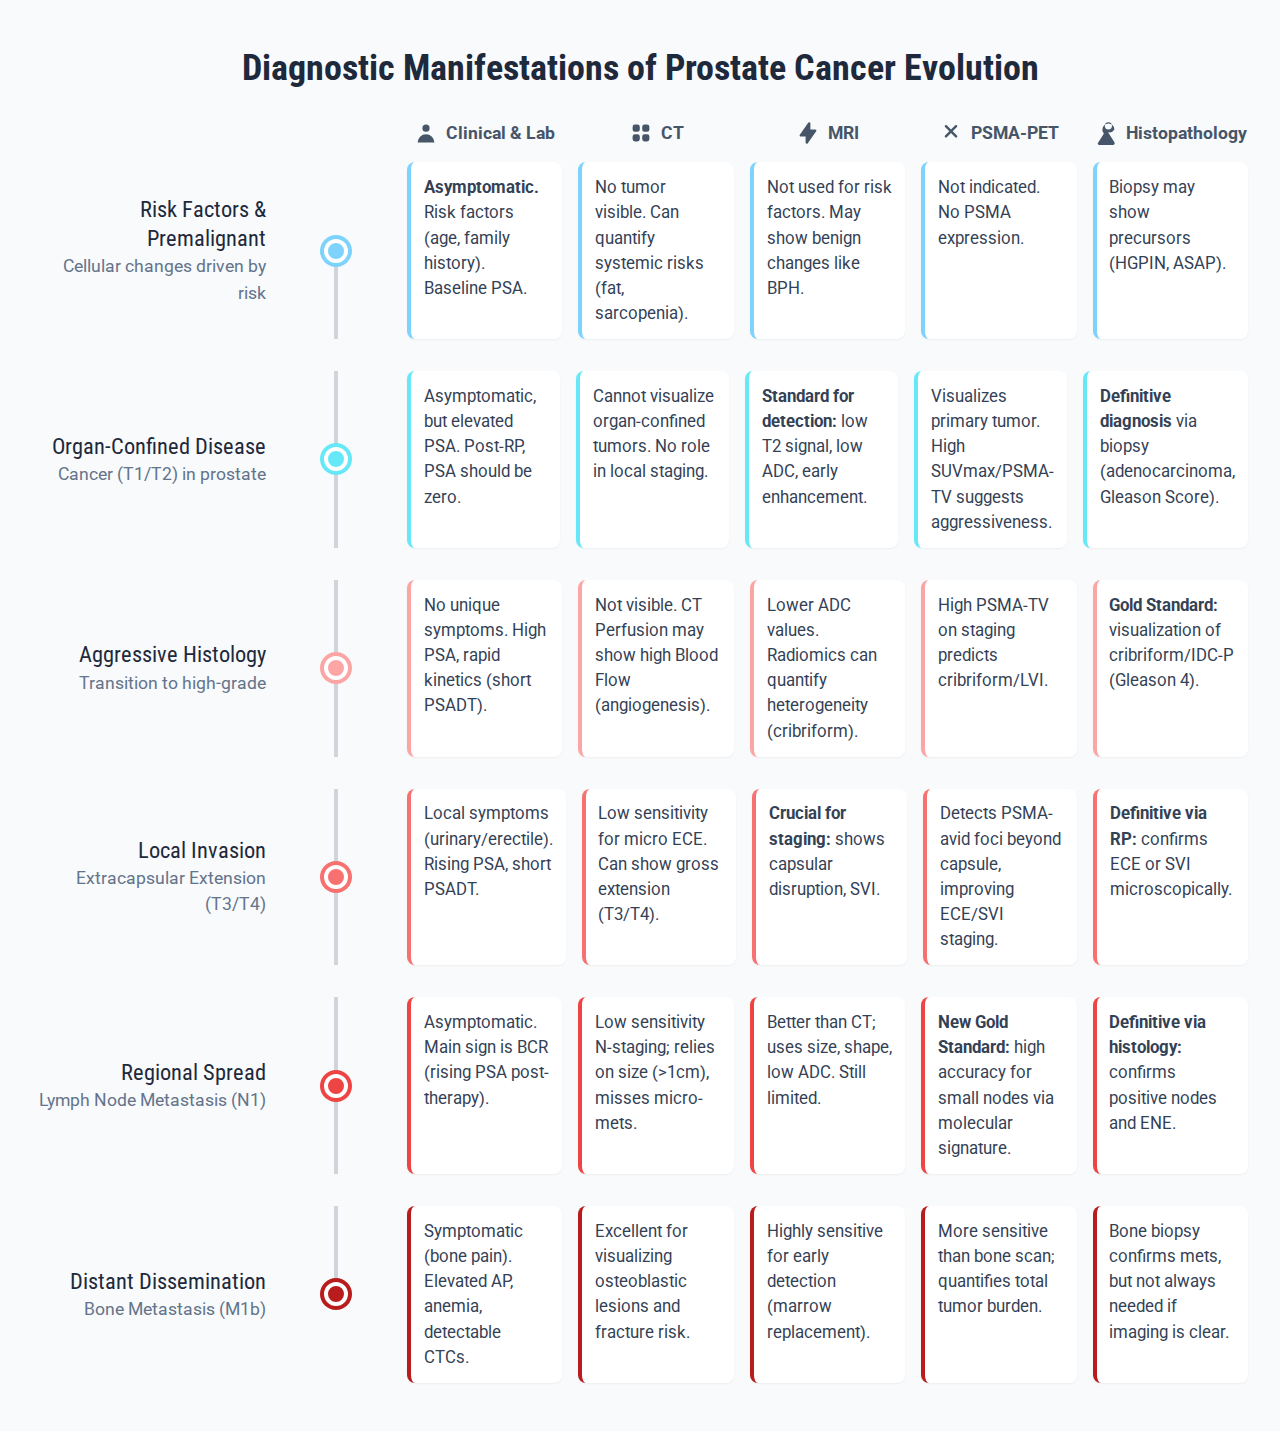
\includegraphics[width=\textwidth]{pe.png}
%     \caption{The natural history of prostate cancer, illustrating the stages our model will learn. The disease evolves based on tumor stage, patient state, and interventions, with information inferred from multiple clinical and imaging modalities. Our hypothesis is moreover that stage of a disease at initial diagnosis is the key to the best futher theraphy.}
%     \label{fig:prostate_evolution}
% \end{figure}

\subsection{Plausibility of the Methodology}
Our methodology is a direct answer to the profound challenges of building trustworthy clinical AI. We aim to design the novel, \textbf{five-stage causal framework proposed in this study}, which deconstructs the immense complexity of prostate cancer progression into a series of well-defined, manageable tasks, \textbf{corresponding to the five stages detailed below}. This modular approach is the key to our project's feasibility: it ensures training stability, enhances model interpretability, and allows us to systematically embed clinical domain knowledge as strong inductive biases. This extensive integration of domain knowledge is crucial for ensuring the model generalizes well beyond its training data. This is achieved by infusing medical knowledge at every level: from using specialized \textbf{ordinal loss functions} that understand clinical severity scales (like PI-RADS) to pre-training temporal models on established \textbf{EAU clinical guidelines} and architecturally separating disease signals from technical confounders. The use of a carefully crafted disentangled latent space is a direct and innovative response to the "curse of dimensionality"; without this approach, reliably training a model on such complex, time-varied, and incomplete data would be practically impossible. Each element of our proposed framework is based on a dual foundation of strong, \textbf{peer-reviewed research} and continuous \textbf{clinician-in-the-loop feedback}, ensuring that our ambitious goals are built on a solid scientific and clinically-validated foundation. This foundation is further strengthened by \textbf{leveraging new, proprietary multicenter patient data} reflecting up-to-date and novel treatment methodologies, alongside rich \textbf{open-source databases} such as \gls{tcga} and ProstateNET from the \gls{eucaim} initiative. This combination of established research and diverse, modern data guides the model to learn the true underlying causal mechanisms of the disease, rather than superficial correlations.



This project will start mainly at a Technology Readiness Level (TRL) of 1 for the general framework, as it involves fundamental research into a new causal AI paradigm. However, for some tasks such as initial data processing and management components, we will begin with TRL 3. This is possible because we will leverage and build upon the tools and basic infrastructure developed in an ongoing, highly complementary, local AI project (see 4.2).




\subsubsection{Stage 1: Building the Bedrock of Clinical Validity with Supervisor Models}
The first stage builds a suite of specialized "supervisor" models. These models act as expert guides, providing strong, clinically-validated signals that will enforce a valid structure on the more complex generative models in subsequent stages. Our team's prior success in developing predictive models from fused clinical and imaging data provides a strong foundation for this work package.
\begin{itemize}
    \item \textbf{Ordinal Classifiers:} For clinical scores with an inherent order (e.g., PI-RADS, TNM stage), standard categorical classifiers are suboptimal. We will implement a \textbf{differential ordinal learning framework} that explicitly encodes the ordered structure by combining a standard categorical loss with a differential ordinal loss, ensuring the model understands that a higher grade implies a worse prognosis \cite{LeeByeon2025}.
    \item \textbf{Censored Survival Regressor:} To predict \gls{ttp}, we will train a survival model that properly handles right-censored data. This will be achieved using a censored regression loss (e.g., Logistic Hazard) combined with a ranking loss regularizer (e.g., SurvRNC) to ensure correct risk ordering in the learned feature representation \cite{GaoLi2019}.
This approach ensures the model generalizes well and produces more clinically plausible counterfactuals \cite{PuglisiAlexander2025}.
\end{itemize}

\begin{figure}[H]
    \centering
    
\includegraphics[width=\textwidth]{dc.png}
    \caption{An infographic summarizing the new data acquisition, curation, and preprocessing framework for the study cohort. It details the inclusion and exclusion criteria for patient selection and outlines the multi-step pipeline for processing clinical, histopathological, and imaging data. The \gls{ehr} is a key source of clinical data.}
    \label{fig:data_curation}
\end{figure}
\subsubsection{Stage 2: Mastering Heterogeneity through Principled Disentanglement}
At the heart of our solution to data heterogeneity is a hierarchical \gls{vae} trained for each imaging modality to learn a disentangled latent space. The key innovation is partitioning this space into four independent, semantically meaningful components: Anatomy ($Z_A$), Disease ($Z_D$), Patient State ($Z_P$), and Style/Confounders ($Z_S$). This separation is enforced through a composite loss function:
$$ \mathcal{L}_{\text{total}} = \mathcal{L}_{\text{VAE}} + \lambda_A \mathcal{L}_{\text{Anatomy}} + \lambda_D \mathcal{L}_{\text{Disease}} + \lambda_I \mathcal{L}_{\text{Disentangle}} $$
The disentanglement is achieved by moving beyond simple $\beta$-VAE approaches. 

Our loss function will apply a \textbf{targeted penalization} of the statistical dependence between latent subspaces. We recognize that some correlations are clinically meaningful (e.g., disease can affect anatomy), while others are spurious. Therefore, the model will be heavily penalized for mutual information between causally independent subspaces (e.g., Disease $Z_D$ and Style $Z_S$, which includes scanner type and data source), while allowing for natural correlations between dependent factors like disease and anatomy. 
This is accomplished by selectively applying a Total Correlation (TC) penalty, ensuring the learned disease representation is invariant to technical artifacts without sacrificing the reconstruction of clinically valid relationships \cite{FragemannArdizzone2022, AbbasiMonadjemi2018, FayCobos2023}. The entire data curation and preprocessing pipeline is visualized in Figure \ref{fig:data_curation}.

\subsubsection{Stage 3: VAE-based Out-of-Distribution Detection for Label Noise Resilience}
To enhance the robustness of our framework against imperfections in data labeling (e.g., for TNM stage or PI-RADS scores), we will incorporate a dedicated VAE-based Out-of-Distribution (OOD) detection mechanism. This additional stage in our methodology is designed to identify atypical or potentially mislabeled data points by analyzing their representation in the latent space. The core principle is that VAEs, when trained on a coherent dataset, learn a compact and structured representation of "normality" \cite{PuglisiAlexander2025,YuanStojanovski2025}. Samples that deviate significantly from this learned normality can be flagged as OOD instances for manual verification by a medical professional.


The methodology is as follows:
\begin{enumerate}
    \item \textbf{Learning a Normality Manifold:} A VAE will be trained on the encoded latent space representations ($Z_D$ and $Z_P$) from our primary disentanglement stage. The VAE's objective, regularized by a Kullback–Leibler Divergence (KLD) loss, is to learn a smooth, continuous manifold that captures the underlying distribution of the in-distribution (ID) data \cite{YuanStojanovski2025,ZhouZhou2025}.
    \item \textbf{Quantifying Deviation:} When a new data sample is processed, its latent representation is passed through the trained VAE. OOD samples are identified through two primary metrics:
    \begin{itemize}
        \item \textbf{Reconstruction Error:} The VAE will struggle to accurately reconstruct latent vectors that lie far from the learned normality manifold. A high reconstruction error serves as a strong indicator of an OOD sample \cite{BiHuang2025,ZhangGe2025}.
        \item \textbf{Latent Space Distance:} OOD samples are hypothesized to lie farther away from the dense clusters of ID samples in the embedded feature space \cite{LiaoHu2025}. We will implement a K-Nearest Neighbors (KNN) based approach to quantify this distance, calculating an OOD score based on the Euclidean distance between a sample's latent representation and its k-th nearest clean neighbor \cite{ZhangGe2025,LiaoHu2025}.
    \end{itemize}
    \item \textbf{Flagging for Expert Review:} Samples exceeding a predefined threshold for either reconstruction error or latent space distance will be automatically flagged. These "atypical" cases, which may represent rare disease presentations, imaging artifacts, or labeling errors, will be presented to our clinical partners for manual review and correction.
\end{enumerate}
By implementing this verification loop, we can proactively identify and correct open-set label noise, which is known to significantly degrade model performance \cite{LiaoHu2025}.  This ensures a higher quality training dataset and ultimately leads to a more robust, reliable, and trustworthy clinical AI.

\subsubsection{Stage 4: Capturing Disease Dynamics with Neural Jump ODEs}
This stage confronts the critical challenge of modeling disease evolution from sparse, multimodal, and irregularly-sampled clinical data. Our solution is a \textbf{\gls{njde}} framework, which is uniquely suited for this task \cite{GwakSim2020}.

\paragraph{Rationale and Latent State Formulation}
Neural Ordinary Differential Equations (NODEs) are powerful because they model system dynamics in continuous time, making them inherently robust to irregular sampling—a defining characteristic of clinical data \cite{GwakSim2020, JohnsonBulgarelli2023, BelogolovskyGreenberg2023}. However, their primary weakness is the extreme computational cost of applying them directly to high-dimensional data like 3D images \cite{WiewelBecher2018, DavisChoromanski2020}. Our approach strategically mitigates this by operating exclusively on the low-dimensional latent spaces learned in Stage 2. This is not just an efficiency gain for training; it is a critical design choice that ensures the model's \textbf{computational feasibility} for inference in a real-world clinical setting. Thanks to the successful disentanglement, we do not need to pass the entire latent space to the temporal model. Instead, by training the NODE only on the most relevant parts—the disentangled \textbf{disease ($Z_D$) and patient state ($Z_P$) components}—we focus the model on learning the dynamics of disease progression itself, making the learning task more tractable and clinically relevant \cite{AshmanSo2020, KberKalisch2023, LosadaTerranova2024}. Crucially, by modeling the evolution of these purified latent vectors, we are not just fitting a curve to data points; we are learning a representation of the underlying causal trajectory of the disease, stripped of observational noise and technical artifacts.

The input for the \gls{njde} is a carefully constructed time series of latent state vectors. For each patient, we define a unified state vector $\mathbf{v}$ that has a fixed shape, representing a concatenation of all possible inputs. The process is as follows:
\begin{enumerate}
    \item \textbf{Unified State Vector Definition:} A canonical tensor shape is defined for a state vector $\mathbf{v}$, which includes dedicated slots for the disease latent code ($Z_D$) and patient state code ($Z_P$) from each imaging modality (\gls{mri}, \gls{pet}, SPECT), and for embeddings of all non-imaging data (PSA, clinical note embeddings, etc.).
    \item \textbf{Time-stamped Sparse Tensor Creation:} For each time point $t_i$ where a patient has data, a new state vector $\mathbf{v}(t_i)$ is created and initialized with zeros. The available data is then placed into its corresponding slot in the tensor. For example, at a time point with a \gls{pet} scan and PSA value, only the $Z_{D_{\text{PET}}}$, $Z_{P_{\text{PET}}}$, and PSA embedding slots are filled, while all other slots remain zero.
    \item \textbf{Anatomy Vector Storage:} The patient-specific anatomy vectors ($Z_A$) from each imaging study are not included in the dynamic state vector but are stored separately, indexed by time, for use in the final image reconstruction stage.
\end{enumerate}
This procedure yields a dataset of sparse, irregularly-sampled latent state vectors, providing a computationally efficient and robust representation of each patient's unique clinical history.

\paragraph{NJDE Training and Dynamics}
The \gls{njde} learns the rules of disease evolution by modeling two phenomena \cite{GwakSim2020}:
\begin{itemize}
    \item \textbf{Continuous Evolution (The NODE):} Between clinical events, the disease state evolves smoothly. This is modeled by a classic NODE that learns the underlying dynamics from the sparse state vectors \cite{BergHasenclever2018}.
    $$ \frac{d\mathbf{v}(t)}{dt} = f(\mathbf{v}(t), t; \psi) \quad \text{for } t \neq t_k $$
    \item \textbf{Discrete Jumps (The Interventions):} At the specific time $t_k$ of a clinical intervention (e.g., radical prostatectomy, initiation of systemic therapies such as \gls{adt} or chemotherapy, or targeted radioligand therapy with $^{\text{177}}\text{Lu-PSMA}$), the continuous evolution is interrupted by a discrete "jump." A separate neural network, $g$, models this instantaneous change to the state vector based on the type of intervention \cite{CuchieroLarsson2019, AbushaqraXue2022}. Crucially, the model is designed to handle multiple, sequential jumps, allowing it to accurately represent a patient's entire treatment history, which may involve several different lines of therapy over time.
    $$ \mathbf{v}^+ = g(\mathbf{v}(t_k), \text{intervention}_k; \phi) \quad \text{for } t = t_k $$
\end{itemize}




This hybrid approach, which explicitly separates the continuous disease course from the rapid, external impacts of clinical interventions, is critical for accurately modeling a patient's journey \cite{GwakSim2020}. The model is trained using a \textbf{leave-one-out strategy} for each patient's time series: given all but one time point, its goal is to predict the complete state vector for the held-out time point. To handle the pervasive missing data, we will first develop a simplified, rule-based decision algorithm in close consultation with our urology partners. This algorithm, based on the \gls{eau} guidelines, will provide a baseline management recommendation even for cases with incomplete data.


The \gls{njde} model will then be pre-trained on the outputs of this decision tree, allowing it to develop an initial, robust understanding of the relationships between patient state, disease status, and appropriate management pathways before being fine-tuned on the full, complex tumour board data. For the fine-tuning stage, we will employ a \textbf{masked loss function}. The loss is calculated only by comparing the predicted values to the ground truth for those elements of the state vector that were actually available (non-zero) at the target time point. This forces the model to learn a probable evolution for every data type, even from a highly incomplete dataset. By distinguishing between smooth progression and intervention-driven shocks, the \gls{njde} learns a more biologically plausible model of the patient's journey.


\subsubsection{Stage 5: Translating Insight into Action: Generative Synthesis, Decision Support, and Structured Reporting}
The final stage translates the model's learned causal dynamics into clinically actionable outputs, evolving the framework from a descriptive tool into an active partner in clinical decision-making. This includes generating high-fidelity images for any time point or counterfactual scenario, with a lightweight Diffusion Model used as a final post-processing step to ensure realism. These visual outputs serve as the intuitive foundation for the system's core decision support capabilities. Apart form visual outputs values for PSA , TNM or time to progression will also be inferred in any requested time point. 
\begin{figure}[H]
    \centering
    
\includegraphics[        trim=5mm 10mm 5mm 10mm, % {left bottom right top}
        clip,                     % This command applies the trim
        width=\textwidth]{ml.png}
    \caption{The proposed multi-stage causal AI framework.}
    \label{fig:ml_framework}
\end{figure}


% \begin{figure}[H]
%     \centering
%     
\includegraphics[        trim=5mm 10mm 5mm 10mm, % {left bottom right top}
%         clip,                     % This command applies the trim
%         width=\textwidth]{ml.png}
%     \caption{The proposed multi-stage causal AI framework.}
%     \label{fig:ml_framework}
% \end{figure}


A key innovation in this stage is the use of clinician interaction patterns as a feedback loop. The framework's user interface will be designed to log all interactions, such as the specific "what-if" questions asked, the counterfactuals generated, and the treatment scenarios explored by the clinician. This interaction data will be analyzed to identify recurring patterns of inquiry, which can provide valuable insights into the clinician's diagnostic and treatment-planning thought process. This information will then be used to personalize the "digital twin's" outputs in two ways:
\begin{itemize}
    \item \textbf{Personalized Explanations:} By understanding the questions a clinician frequently asks about a particular type of case, the system can proactively generate the most relevant counterfactuals and visualizations, tailoring its explanations to the user's specific cognitive workflow.
    \item \textbf{Adaptive Patient-Facing Visualizations:} The system will use the insights from clinician interactions to create simplified, more intuitive visualizations of the expected disease progression for patients. By knowing what aspects of the data are most critical for decision-making, the system can generate clearer, more focused graphical timelines and outcome predictions, helping patients to better understand their condition and treatment options.
\end{itemize}


Crucially, the framework will function as a \textbf{Treatment-Choice Helper}. Leveraging the \gls{njde} from Stage 3, the system will simulate multiple future patient trajectories, each conditioned on a different potential treatment intervention and timing. By comparing these simulated outcomes, the model can identify the therapeutic strategy that is explicitly optimized to \textbf{maximize the expected time to progression}. This transforms the "what-if" capability from a simple explanatory tool into a powerful engine for data-driven treatment planning.

All insights are then consolidated into automatically generated structured reports using a \textbf{Transformer-based decoder}. These reports will integrate prognostic simulations, present the comparative effectiveness of different treatment options, and culminate in a data-driven recommendation. This directly addresses the clinical need for clear, consistent, and efficient documentation \cite{JorgHalfmann2023, SacoranskyKwan2024}, while providing clinicians with novel, data-driven strategies for patient management. The project team's experience in creating LLM-based support apps and and GUIs from structured reports is key to ensuring this complex information is presented in an intuitive and actionable format. The framework is summarized in Figure \ref{fig:ml_framework}



\subsubsection{Uncertainty Quantification and Explainable AI}
A key feature for clinical trust is the model's ability to quantify its own uncertainty. Our \gls{vae}-based architecture is intrinsically probabilistic and allows for robust uncertainty quantification. We will employ two complementary methods:
\begin{itemize}
    \item \textbf{Latent Space Sampling:} For a given input, we will draw multiple samples from its learned latent distribution. The variance in the resulting predictions will serve as a robust measure of the model's epistemic uncertainty \cite{BustinMeyer2025}.
    \item \textbf{Direct Variance Utilisation:} The variance vector $\sigma^2$ produced by the \gls{vae} encoder is a direct indicator of feature-level uncertainty. We will concatenate this variance vector to the mean vector as a direct input to downstream models, allowing them to learn to depend more on high-confidence features \cite{FriedrichFrisch2024}.
\end{itemize}

Morover this possibility of repeated executions will also show what entries in structural report are shown consistently by the model and which are not - flagging potential problematic areas and reducing risk of undetected \textbf{hallucinations}.  Similar mechanism will work for managament suggestions. 

The proposed framework is explainable by design supplying counterfactual reasoning, but for stage 1 classifiers particularly other techniques like Shapley values or Grad-CAM will be used. 

\subsubsection{Quantitative Metrics}
Model performance will be assessed using a comprehensive suite of metrics tailored to each sub-task, presented in a clear "Metric - What it measures - Why it's relevant" format:
\begin{itemize}
    \item \textbf{Supervisor Model Performance:}
        \begin{itemize}
            \item \textbf{Classification (Accuracy, \gls{auc}, F1-Score):} These metrics measure the model's ability to correctly classify categorical variables like TNM stage and PI-RADS score. They are relevant for assessing the model's fundamental diagnostic accuracy.
            \item \textbf{Survival Regression (\gls{cindex}, \gls{mae}):} These metrics measure the model's ability to predict \gls{ttp}. They are relevant for assessing the model's prognostic accuracy.
        \end{itemize}
    \item \textbf{Generative Model Performance:}
        \begin{itemize}
            \item \textbf{Image Generation Quality (\gls{fid}, \gls{ssim}):} These metrics measure the realism and fidelity of the generated images. They are relevant for ensuring the clinical plausibility of the model's outputs.

        \end{itemize}
\end{itemize}

\subsubsection{Component-Wise and Joint Validation Strategy}
Our validation strategy is designed to rigorously test each component of the framework in isolation before assessing the performance of the integrated system. This staged approach, detailed below, ensures that each module is robust and reliable before it is incorporated into the full clinical workflow.

\paragraph{Stage 0: Data Quality Assurance}
For \textbf{Isolated Testing}, the VAE-based OOD detection model will be evaluated on its ability to distinguish between a clean validation set and a validation set seeded with synthetic anomalies. Metrics will include AUC for OOD detection. This stage validates the quality of the initial curated dataset (\textbf{D1.1}). For \textbf{Joint Testing}, the flagged outliers will be reviewed by clinical experts. The percentage of clinically-confirmed outliers will serve as a measure of the system's real-world effectiveness. The impact of this cleaning step will be measured by the performance improvement of all downstream models.

\paragraph{Stage 1: Supervisor Models}
For \textbf{Isolated Testing}, each model (ordinal classifiers, survival regressor, etc.) will be tested independently against its specific ground truth using standard metrics (Accuracy, AUC, C-index). Success is formally verified by \textbf{Milestone M2}, with models delivered in \textbf{D2.1}. For \textbf{Joint Testing}, the outputs of the supervisor models will be used as inputs for the VAEs in Stage 2. The quality of the VAE's disentanglement will serve as an indirect measure of the supervisor models' performance.

\paragraph{Stage 2: Causal VAEs}
For \textbf{Isolated Testing}, the VAEs will be evaluated on their ability to generate realistic images (measured by FID, SSIM) and to successfully disentangle the latent space. Success is verified by \textbf{Milestones M3 and M7}. Models are delivered in \textbf{D3.1}. For \textbf{Joint Testing}, the disentangled latent vectors from the VAEs will be used as inputs for the NJDE model in Stage 3. The NJDE's predictive accuracy and calibration will be used to assess the quality of the learned representations.

\paragraph{Stage 3: Neural Jump ODE}
For \textbf{Isolated Testing}, the NJDE will be tested on its ability to accurately predict future latent states from a given history, using a masked loss function to handle missing data. Success is verified by \textbf{Milestone M4}. The final model is delivered in \textbf{D4.1}. For \textbf{Joint Testing}, the predicted latent states from the NJDE will be passed to the VAE decoders to generate future images. The quality of these generated images will be assessed both quantitatively (FID, SSIM) and qualitatively by clinicians.

\paragraph{Stage 4: Full Framework}
For \textbf{Isolated Testing}, the complete, end-to-end framework will be evaluated in a simulated clinical environment. This includes testing the user interface and the generation of structured reports. For \textbf{Joint Testing}, a comprehensive clinical plausibility study will be conducted to assess real-world utility. Crucially, we will perform a series of \textbf{ablation studies} to quantify the impact of our knowledge integration. The final integrated system is validated against \textbf{Milestones M5 and M6}, with results summarized in the final validation report (\textbf{D5.1}).

Moreover, The Physikalisch-Technische Bundesanstalt (PTB), Braunschweig, will serve as a neutral quality partner for metrology, reference datasets, uncertainty/robustness metrics, and \textbf{Medical Device Regulation (MDR)}/\textbf{AI-Act}-ready evaluation within a \textbf{Testing and Experimentation Facility (TEF)}-aligned framework.



\subsubsection{Clinical Plausibility and Workflow Integration Study}
Beyond quantitative metrics, a practical, clinician-in-the-loop study is essential to assess the model's real-world utility and trustworthiness.

First, we will \textbf{assess explanation faithfulness and plausibility}. To evaluate the quality of our generated explanations (\gls{xai}), we will conduct a two-part human-grounded study with radiologists and oncologists. For \textbf{qualitative plausibility}, clinicians will be presented with a series of cases, each including an original image and its corresponding model-generated counterfactual. They will score the counterfactuals on a Likert scale for: 1) \textbf{Clinical Plausibility} (Does it appear realistic?) and 2) \textbf{Usefulness for Explanation} (Does it provide a clear reason for the model's prediction?) for \textbf{quantitative faithfulness} .



Second, we will \textbf{measure workflow improvement and decision support utility} through a comparative workflow study. A control group of clinicians will review patient cases using traditional methods, while an experimental group will use our system's auto-generated structured reports and prognostic visualizations. We will measure several \textbf{workflow metrics}, including: 1) \textbf{Efficiency} (time to extract key information), 2) \textbf{Accuracy and Concordance} (inter-rater agreement compared to an expert-defined ground truth), and 3) \textbf{User Satisfaction} (using the System Usability Scale). For the \textbf{Treatment-Choice Helper} component, we will evaluate its \textbf{recommendation metrics} against a gold standard (e.g., tumor board consensus, for which we will report \textbf{inter-rater agreement}). These metrics will include \textbf{Top-k Accuracy} (k=1, 3), and \textbf{Recall}. 




\subsubsection{Statistical Rigor and Robustness Analysis}
All validation will adhere to rigorous statistical principles to ensure the reliability and generalizability of our findings.
\begin{itemize}
       \item \textbf{Statistical Testing:} All reported metrics where applicable will be accompanied by \textbf{95\% confidence intervals}. Comparisons between models (e.g., for \gls{auc}) will use appropriate statistical tests, such as the \textbf{DeLong test}, with \textbf{multiplicity correction} (e.g., Holm-Bonferroni). We will use a \textbf{locked external test set} for final validation, with operating point thresholds pre-specified to avoid post-hoc bias. We moreover intend to test framework on data from clinic that had not participated in training of the models so as external validation.
    
    \item \textbf{Robustness and Fairness:} To ensure robustness, we will stress-test the model against various patterns of missing data. To ensure \textbf{transportability}, we will report key metrics on a \textbf{per-site basis} and identify \textbf{worst-group performance}.
    
    \item \textbf{Subgroup and Bias Analysis:} We will conduct a comprehensive \textbf{subgroup analysis}, reporting key metrics (e.g., \gls{auc}, \gls{cindex}) and \textbf{calibration gaps} across clinically relevant strata (e.g., age, comorbidity, hospital site). We will quantify any performance disparities, such as gaps in True Positive Rates (TPR), to proactively identify and mitigate potential biases.
\end{itemize}


\subsubsection{Research Data Management and FAIR Principles}
All research data and other research outputs generated in this project will be managed in line with the FAIR (Findable, Accessible, Interoperable, Reusable) principles. A detailed Data Management Plan (DMP) will be developed as a formal deliverable by month 6 of the project and will be updated as needed. Our management strategy is as follows:


\begin{itemize}
    \item \textbf{Types of Data and Estimated Size:} The project will generate and collect several types of research data, including observational clinical data from \gls{ehr}s, numerical data (e.g., PSA values), and extensive 3D medical imaging data (e.g.\gls{mri}, \gls{pet}, \gls{ct}). We will use data from the regional State Cancer Registries (e.g., the Saxony-Anhalt Cancer Registry and other German state cancer registries) to obtain comprehensive information on patient outcomes, including completeness of follow-up, progression-free survival (PFS), and overall survival (OS) - PFS will be also derived from EHR–imaging linkages due to registry limitations and latency. We will also generate derived data, such as disentangled latent space vectors and synthetic images. The total estimated size of the curated dataset is expected to be approximately 200 Terabytes.
\end{itemize}




\begin{itemize}

    \item \textbf{Findability:} To ensure findability, curated and anonymized datasets intended for public release will be deposited in a trusted repository, such as the \gls{eucaim} platform, and assigned a persistent Digital Object Identifier (DOI). All software and models will be version-controlled and made available through our public GitHub repository.
    \item \textbf{Accessibility:} In compliance with GDPR and patient privacy, the raw clinical data cannot be made fully open access. However, we are committed to Open Science. Anonymized, derived datasets will be made available to the scientific community upon project completion. Access to restricted data for the purposes of verification will be granted under secure conditions and governed by formal Data Sharing Agreements (DSAs). All publications will be Gold Open Access.
    \item \textbf{Interoperability:} We will use established standards to ensure interoperability. Imaging data will be managed in the DICOM format. For clinical data, we will leverage standards such as the OMOP-CDM and EUCAIM hyper ontology to facilitate harmonization and integration, as outlined in WP1. Metadata will be provided in a standardized, machine-readable format.
    \item \textbf{Reusability:} To maximize reusability, all software developed within the project will be released under a permissive open-source license (e.g., Apache 2.0). The shared, anonymized datasets will be released under a Creative Commons license (e.g., CC BY-NC 4.0) to encourage non-commercial research and re-use.
    \item \textbf{Curation and Responsibility:} The project's dedicated Data Scientist, under the supervision of the PI and in coordination with the institutional Data Integration Center, will be responsible for all aspects of data management, quality assurance, and curation. This includes overseeing the data pipeline, ensuring data integrity, and managing the long-term storage and preservation of the project's digital assets.
\end{itemize}
% \subsection{Component-Wise and Joint Validation Strategy, linked to Milestones and Deliverables.}
% \paragraph{Stage 0: Data Quality Assurance}
% For \textbf{Isolated Testing}, the VAE-based OOD detection model will be evaluated on its ability to distinguish between a clean validation set and a validation set seeded with synthetic anomalies. Metrics will include AUC for OOD detection. This stage validates the quality of the initial curated dataset (\textbf{D1.1}). For \textbf{Joint Testing}, the flagged outliers will be reviewed by clinical experts. The percentage of clinically-confirmed outliers will serve as a measure of the system's real-world effectiveness. The impact of this cleaning step will be measured by the performance improvement of all downstream models.

% \paragraph{Stage 1: Supervisor Models}
% For \textbf{Isolated Testing}, each model (ordinal classifiers, survival regressor, etc.) will be tested independently against its specific ground truth using standard metrics (Accuracy, AUC, C-index). Success is formally verified by \textbf{Milestone M2}, with models delivered in \textbf{D2.1}. For \textbf{Joint Testing}, the outputs of the supervisor models will be used as inputs for the VAEs in Stage 2. The quality of the VAE's disentanglement will serve as an indirect measure of the supervisor models' performance.

% \paragraph{Stage 2: Causal VAEs}
% For \textbf{Isolated Testing}, the VAEs will be evaluated on their ability to generate realistic images (measured by FID, SSIM) and to successfully disentangle the latent space. Success is verified by \textbf{Milestones M3 and M7}. Models are delivered in \textbf{D3.1}. For \textbf{Joint Testing}, the disentangled latent vectors from the VAEs will be used as inputs for the NJDE model in Stage 3. The NJDE's predictive accuracy and calibration will be used to assess the quality of the learned representations.

% \paragraph{Stage 3: Neural Jump ODE}
% For \textbf{Isolated Testing}, the NJDE will be tested on its ability to accurately predict future latent states from a given history, using a masked loss function to handle missing data. Success is verified by \textbf{Milestone M4}. The final model is delivered in \textbf{D4.1}. For \textbf{Joint Testing}, the predicted latent states from the NJDE will be passed to the VAE decoders to generate future images. The quality of these generated images will be assessed both quantitatively (FID, SSIM) and qualitatively by clinicians.

% \paragraph{Stage 4: Full Framework}
% For \textbf{Isolated Testing}, the complete, end-to-end framework will be evaluated in a simulated clinical environment. This includes testing the user interface and the generation of structured reports. For \textbf{Joint Testing}, a comprehensive clinical plausibility study will be conducted to assess real-world utility. Crucially, we will perform a series of \textbf{ablation studies} to quantify the impact of our knowledge integration. The final integrated system is validated against \textbf{Milestones M5 and M6}, with results summarized in the final validation report (\textbf{D5.1}).

% \begin{longtable}[H]
%     \centering
%     \caption{Component-Wise and Joint Validation Strategy, linked to Milestones and Deliverables.}
%     \label{tab:validation_strategy}
%     \small
%     \begin{tabular}{p{0.25\textwidth} p{0.35\textwidth} p{0.35\textwidth}}
%         \toprule
%         \textbf{Component/Stage} & \textbf{Isolated Testing} & \textbf{Joint Testing} \\
%         \midrule
%         \textbf{Stage 0: Data Quality Assurance} & The VAE-based OOD detection model will be evaluated on its ability to distinguish between a clean validation set and a validation set seeded with synthetic anomalies. Metrics will include AUC for OOD detection. This stage validates the quality of the initial curated dataset (\textbf{D1.1}). & The flagged outliers will be reviewed by clinical experts. The percentage of clinically-confirmed outliers will serve as a measure of the system's real-world effectiveness. The impact of this cleaning step will be measured by the performance improvement of all downstream models. \\
%         \addlinespace
%         \textbf{Stage 1: Supervisor Models} & Each model (ordinal classifiers, survival regressor, etc.) will be tested independently against its specific ground truth using standard metrics (Accuracy, AUC, C-index). Success is formally verified by \textbf{Milestone M2}, with models delivered in \textbf{D2.1}. & The outputs of the supervisor models will be used as inputs for the VAEs in Stage 2. The quality of the VAE's disentanglement will serve as an indirect measure of the supervisor models' performance. \\
%         \addlinespace
%         \textbf{Stage 2: Causal VAEs} & The VAEs will be evaluated on their ability to generate realistic images (measured by FID, SSIM) and to successfully disentangle the latent space. Success is verified by \textbf{Milestones M3 and M7}. Models are delivered in \textbf{D3.1}. & The disentangled latent vectors from the VAEs will be used as inputs for the NJDE model in Stage 3. The NJDE's predictive accuracy and calibration will be used to assess the quality of the learned representations. \\
%         \addlinespace
%         \textbf{Stage 3: Neural Jump ODE} & The NJDE will be tested on its ability to accurately predict future latent states from a given history, using a masked loss function to handle missing data. Success is verified by \textbf{Milestone M4}. The final model is delivered in \textbf{D4.1}. & The predicted latent states from the NJDE will be passed to the VAE decoders to generate future images. The quality of these generated images will be assessed both quantitatively (FID, SSIM) and qualitatively by clinicians. \\
%         \addlinespace
%         \textbf{Stage 4: Full Framework} & The complete, end-to-end framework will be evaluated in a simulated clinical environment. This includes testing the user interface and the generation of structured reports. & A comprehensive clinical plausibility study will be conducted to assess real-world utility. Crucially, we will perform a series of \textbf{ablation studies} to quantify the impact of our knowledge integration. The final integrated system is validated against \textbf{Milestones M5 and M6}, with results summarized in the final validation report (\textbf{D5.1}). \\
%         \bottomrule
%     \end{tabular}
% \end{longtable}

\begin{longtable}{p{0.95\textwidth}}
\toprule
\textbf{Methodological Risk Analysis and Mitigation Strategies} \\
\midrule
\endfirsthead
\endhead

\textbf{Risk 1 (Conceptual): High Project Complexity \& Low Starting TRL} \\
\textit{Likelihood: Medium, Impact: High}\\
\textbf{Risk:} The project's core ambition to create a comprehensive causal framework begins at TRL 1, which signifies fundamental research with a high inherent risk of not achieving the envisioned breakthrough. \\
\textbf{Mitigation:} The project's complexity is managed by deconstructing it into a modular, five-stage framework. Each component is based on methods with established, published implementations, which reduces technical risk. We further mitigate this by building upon a TRL 3 foundation for data processing derived from the SIKIT project, de-risking the initial phases.\\
\textbf{Expected Effect:} This structured, modular approach makes the project tractable and allows for clear progress monitoring, while leveraging existing projects provides a solid technical bedrock, increasing the probability of success. \\
\addlinespace

\textbf{Risk 2 (Operational): Training Instability and Data Scalability} \\
\textit{Likelihood: High, Impact: High} \\
\textbf{Risk:} The complexity of the multi-stage framework could lead to unstable training dynamics, particularly when scaling to large, heterogeneous datasets. This could hinder model convergence and reliability. \\
\textbf{Mitigation:} We will implement a sequential, multi-stage training framework where each component is trained and validated independently before being integrated. The modular design, managed through WP2, WP3, and WP4, allows for isolated testing, fine-tuning, and troubleshooting. \\
\textbf{Expected Effect:} This approach de-risks the development process, reduces the likelihood of system-wide failure, stabilizes training, and facilitates a controlled, scalable integration of the final model. \\
\addlinespace

\textbf{Risk 3 (Operational): Generalizability and Overfitting} \\
\textit{Likelihood: Medium, Impact: High} \\
\textbf{Risk:} The model might learn spurious correlations specific to the training data (e.g., scanner-specific artifacts), leading to poor generalization to new, unseen data from other clinical centers. \\
\textbf{Mitigation:} Our core strategy is the principled disentanglement in WP3, which is designed to separate true biological signals from site-specific confounders. This is reinforced by using diverse, multi-center data (WP1) and incorporating strong, clinically-validated inductive biases (e.g., ordinal losses in WP2). \\
\textbf{Expected Effect:} This will result in a more robust and generalizable model that learns the underlying causal mechanisms of the disease, rather than superficial data patterns, ensuring its clinical utility across different healthcare settings. \\
\addlinespace

\textbf{Risk 4 (Operational): Performance with Incomplete and Heterogeneous Data} \\
\textit{Likelihood: Medium, Impact: High}\\
\textbf{Risk:} Real-world clinical data is inherently sparse, incomplete, and irregularly sampled. This could prevent the model from learning the complete, longitudinal patient trajectory, leading to inaccurate predictions. \\
\textbf{Mitigation:} The Neural Jump ODE architecture (WP4) is specifically chosen for its inherent ability to handle sparse and irregular time-series data. We will pre-train the model on a rule-based system derived from clinical guidelines and then fine-tune it using a masked loss function, which allows the model to learn from all available data points without being penalized for missingness. \\
\textbf{Expected Effect:} This ensures that the model can effectively leverage the full patient history, even when data is incomplete, leading to more accurate and robust trajectory modeling. \\

\textbf{Risk (Operational): Insufficient Computational Resources} \\
\textit{Likelihood: Medium, Impact: Medium} \\
\textbf{Risk:} The available on-premises GPU resources, while sufficient for core development, may become a bottleneck for the extensive hyperparameter tuning and large-scale experiments required by the complex VAE (WP3) and NJDE (WP4) models, potentially limiting the exploration of model architectures. \\
\textbf{Mitigation:} We will implement a tiered computational strategy. 1) In-house resources will be prioritized for initial development and training on sensitive data. 2) We will actively apply for supplemental compute time from EuroHPC (We already have experience with similar system having support of KISSKI in SIKIT project \cite{gwdgKISSKIService}  ), as planned, for large-scale tuning and final model training. 3) We will enforce efficient coding practices, such as mixed-precision training and model optimization, to maximize the utility of all available resources. \\
\textbf{Expected Effect:} This approach ensures core development proceeds unhindered while securing a clear path to the high-performance computing required for large-scale optimization, preventing computational power from limiting the project's final performance. \\
\addlinespace
\bottomrule

\end{longtable}

\paragraph{Compliance with the EU Artificial Intelligence Act}
The proposed framework is designed from the ground up to align with the principles of trustworthy AI and to comply with the requirements for high-risk AI systems as laid down in the Regulation (EU) 2024/1689 (the "AI Act"). As a system intended for use in medical diagnosis and to guide treatment, it is classified as a \textbf{high-risk AI system} under Annex III of the Act. Our methodology directly addresses the core obligations for such systems. For instance, our project management (WP7) will implement a continuous, iterative \textbf{Risk Management System (Article 9)} through a dedicated Risk Register established at the project's outset (M1). \textbf{Data and Data Governance (Article 10)} is a cornerstone of WP1, where we will use relevant, representative datasets and proactively implement measures to detect and mitigate potential biases. The system is designed as a decision support tool to ensure \textbf{Human Oversight (Article 14)}, augmenting, not replacing, clinical experts. The framework's ability to generate counterfactual explanations is a direct implementation of the \textbf{Transparency requirements (Article 13)}, and we will maintain comprehensive \textbf{Technical Documentation (Article 11)} and implement automatic logging for \textbf{Record-Keeping (Article 12)}. Finally, WP5 is dedicated to the rigorous validation of \textbf{Accuracy, Robustness, and Cybersecurity (Article 15)}, ensuring the model is resilient and secure.

\paragraph{Gender Dimension and Open Science Practices}
This project is committed to upholding the principles of gender equality and open science. Due to the specific focus on prostate cancer, the sex/gender dimension is not directly applicable to the biological research content; however, we are fully committed to heterogeneous (age, nationality, stage of the disease) patient groups in the training and evaluation cohorts and promote gender equality in our team composition also ensuring equal opportunities in recruitment. 

\textbf{Open Science}
Our commitment to Open Science is central to our methodology and includes making all peer-reviewed publications Gold Open Access, managing data according to FAIR principles, contributing anonymized datasets to the \gls{eucaim} platform, and releasing all developed software under a permissive open-source license. We will publish eventual negative results and recommendations to de-risk portfolio replication and accelerate European standard-setting. 

\section{Impact}
\subsection{Potential impact }

Prostate cancer (PCa) represents a paramount public health challenge, ranking as the second most common cancer in men worldwide \cite{CaraccioloCastello2024,DulleaOSullivan2025}. In 2020 alone, over 1.4 million new cases were diagnosed globally, and it stands as the fifth leading cause of cancer-related death among men, responsible for approximately 375,000 deaths that year \cite{CereserEvangelista2023,GammelSolari2024,DharCendejasGomez2024}. The epidemiological trajectory is alarming, with projections indicating that the number of cases will more than double to 2.9 million by 2040, driven largely by an aging global population \cite{UdovicichJia2025,SungFerlay2021}.
Beyond the statistics, the human cost is immense, with millions of men and their families affected by the physical and psychological toll of the disease and its treatment \cite{NardoneMarmorino2024}.

Our project directly addresses this urgent societal and economic challenge by proposing a transformative technology with the potential to generate significant, quantifiable impact across multiple domains as described below.

\subsubsection{Scale and Significance of Impact}

The primary impact of our project will be a paradigm shift in PCa management, moving from a reactive, population-based approach to a proactive, personalized, and predictive model of care. The scale of this impact is defined by the sheer prevalence of the disease. The successful implementation of our AI-driven "digital twin" has the potential to improve outcomes for a significant proportion of the nearly half a million men diagnosed with PCa in Europe each year.

\begin{itemize}

    \item \textbf{Improved Clinical Decision-Making and Patient Outcomes:} A key benefit of our framework is its ability to provide highly accurate, patient-specific prognostic forecasts. For men with localized disease, this can mean the difference between unnecessary, life-altering treatments and confident active surveillance. The model will directly support clinicians in complex decisions, such as determining the optimal moment to transition from active surveillance to a more aggressive strategy like $^{177}$Lu-PSMA therapy or chemotherapy. Studies have shown that up to 50\% of men with low-risk PCa who undergo radical prostatectomy may be overtreated \cite{HeijnsdijkWever2012}, leading to significant side effects such as incontinence and erectile dysfunction. Our model, by providing a more granular risk assessment, aims to reduce this overtreatment rate. Conversely, for high-risk patients, the model will enable earlier and more aggressive intervention.


    \item \textbf{Enhanced Patient Autonomy and Awareness:} Our project empowers patients by transforming abstract data into intuitive, visual simulations of their potential disease trajectories. This approach enhances patient awareness and understanding of their own condition, fostering greater autonomy in shared decision-making. By making the reasoning behind clinical recommendations more transparent, we aim to improve patient compliance with treatment plans and strengthen the physician-patient relationship.


\item \textbf{Virtual Intervention Simulation:} The proposed framework will address the current limitations in clinical guidelines, particularly the uncertainty surrounding the integration of new imaging modalities like \gls{psma}-\gls{pet}. By creating a digital model of the patient and the disease, our system will be able to simulate virtual interventions and generate research hypotheses. This capability will be crucial for designing targeted and efficient clinical trials to establish how to best use new diagnostic information, ultimately saving resources and reducing patient risk.

    \item \textbf{Enhanced Efficiency and Cost Savings:} The economic impact extends beyond reducing unnecessary treatments. Our framework's ability to automate the generation of structured radiological reports is projected to reduce the time radiologists spend on documentation up to \textbf{24\%} per case \cite{Acosta_2024}. This translates to a significant productivity gain. Furthermore, by accelerating clinical research through in-silico trials, our platform can help reduce the enormous cost of pharmaceutical R\&D. A recent analysis suggests that AI-driven tools could reduce the cost of bringing a new oncology drug to market.

    \item \textbf{Societal Benefits and Quality of Life:} The societal impact is profound. For patients, avoiding overtreatment means preserving a higher quality of life, free from debilitating side effects. For the healthcare system, a more efficient and effective PCa care pathway means a more sustainable use of resources. We estimate that the widespread adoption of our technology could lead to a significant reduction in the overall cost of PCa care in the EU.

    
\end{itemize}

\subsubsection{Pathways to Impact}

Our pathway to achieving this impact is built on a robust, multi-faceted strategy that combines open science with targeted commercial exploitation and deep engagement with the clinical community.

\begin{itemize}
    \item \textbf{Dissemination and Open Science:} The core AI framework and all associated software will be released under a permissive open-source license, fostering a vibrant ecosystem of innovation. We will publish our findings in high-impact, open-access journals and present at leading international conferences. Anonymized, curated datasets will be contributed to the European Cancer Imaging Initiative (EUCAIM), creating a lasting resource for the research community. This open approach is the fastest and most effective way to establish our framework as a new European standard.

    \item \textbf{Clinical Integration and Adoption:} We will work hand-in-hand with our clinical partners to develop a user-friendly, intuitive interface that seamlessly integrates into existing hospital workflows (e.g., PACS and EHR systems). Annual workshops with a dedicated Clinical Advisory Board will ensure the tool is continuously refined based on real-world feedback.

  \item \textbf{Commercial Exploitation:} The primary route to market will be through a future spin-off company. This entity will provide enterprise-grade versions of the software compliant with medical device regulations (such as Regulation (EU) 2017/745 - MDR), including thorough external clinical validation to generate the necessary clinical evidence demonstrating safety and performance for CE marking. These validated versions will come with long-term support. Consultancy services for adapting the framework to other diseases will also be offered. This dual open-source/commercial model ensures both broad accessibility and a sustainable, regulatory-compliant path to market.
\end{itemize}

\subsubsection{Barriers to Impact and Mitigation Strategies}

We recognize that the path to impact is not without its challenges. We have identified several potential barriers and have developed proactive mitigation strategies for each.

\begin{itemize}
    \item \textbf{Barrier 1: Regulatory and Ethical Hurdles:} As a high-risk AI system, our framework will be subject to rigorous regulatory scrutiny under the EU AI Act.
    \begin{itemize}
        \item \textbf{Mitigation:} Our project is designed from the ground up for compliance. We will maintain comprehensive technical documentation, implement robust risk management systems, and ensure human-in-the-loop oversight. Our commitment to transparency and explainability, through features like counterfactual image generation, directly addresses the "right to explanation" and will be crucial for gaining regulatory approval and clinical trust.
    \end{itemize}

    \item \textbf{Barrier 2: Data Heterogeneity and Generalizability:} A model trained on data from a few centers may not generalize well to the diverse healthcare landscape of Europe.
    \begin{itemize}
        \item \textbf{Mitigation:} This is a core technical challenge that we address directly with our principled disentanglement methodology. By architecturally separating true disease signals from site-specific confounders (e.g., scanner type), we are building a model that is robust to data heterogeneity by design. We will also validate our model on a diverse, multi-center dataset to rigorously test its generalizability.
    \end{itemize}

    \item \textbf{Barrier 3: Clinical Inertia and Adoption:} Even the most powerful tool will have no impact if it is not adopted by clinicians.
    \begin{itemize}
        \item \textbf{Mitigation:} Our deep, continuous engagement with clinical partners is our primary mitigation strategy. By involving end-users throughout the development process, we ensure the tool is not just technically advanced but also clinically relevant, intuitive, and genuinely useful in day-to-day practice. The automated reporting feature is a key driver for adoption, as it provides an immediate, tangible benefit in terms of workflow efficiency.
    \end{itemize}
\end{itemize}

By proactively addressing these potential barriers, we are confident that we can successfully translate our cutting-edge research into a transformative technology that will have a lasting and positive impact on the lives of millions of people across Europe.

\subsection{Innovation potential}
Our strategy for translating research results into tangible innovations is built on a dual approach that combines open dissemination with targeted commercial exploitation, ensuring that we both contribute to the public good and create a sustainable path to market.

\paragraph{Exploitation and IP Strategy}
Our intellectual property strategy is designed to maximize both impact and innovation potential. The core causal framework and all related code will be released under a permissive open-source license (e.g., Apache 2.0) to encourage widespread adoption and establish it as a European standard. The primary route for commercial exploitation will be through a potential future spin-off company. This entity would offer value-added services built upon the open-source foundation, such as:
\begin{itemize}
    \item \textbf{Enterprise-Grade Deployment:} Providing validated, production-ready versions of the software with long-term support, tailored for integration into hospital IT systems.
    \item \textbf{Specialized Model Development:} Offering consultancy services to adapt and fine-tune the framework for other cancers or specific clinical use-cases.
    \item \textbf{Cloud-Based Platform:} Developing a secure, cloud-based "AI-as-a-Service" platform to provide easy access to the technology for smaller clinics or research groups without the resources for local deployment.
\end{itemize}
A key innovation that underpins the reliability of our entire framework is the integration of a sophisticated \textbf{VAE-based Out-of-Distribution (OOD) detection mechanism}. While OOD detection is an active area of research, its application to proactively identify and mitigate label noise (for example errors in human derived TNM ) in complex, real-world clinical datasets is a significant novelty. This goes beyond standard data cleaning; it is an integrated quality assurance loop that uses the model's own understanding of "normality" to flag suspicious data points for expert review. By building this self-correcting capability directly into our data pipeline, we are not only developing a more robust and trustworthy AI, but also creating a novel methodology for semi-supervised data curation that can be adopted by the wider medical AI community. This directly addresses a fundamental bottleneck in the development of clinical AI: the reliance on imperfect, manually annotated data.

This model allows us to protect the commercial potential of these services (background IP) while ensuring the core technology (foreground IP) remains open, creating a virtuous cycle of community-driven improvement and commercially-supported stability. This dual approach is a highly adequate measure for protecting our results while maximizing their reach and impact, facilitating the future translation of our research into tangible innovations.

\paragraph{Involving and Empowering Key Actors}
We will actively involve and empower the key actors needed to translate our research into innovation through concrete, planned activities:
\begin{itemize}
    \item \textbf{Clinicians and Hospitals:} Our close collaboration with university hospitals ( for example from Halle) will be operationalized through \textbf{annual project workshops} and the establishment of a \textbf{Clinical Advisory Board}. This ensures the technology is developed with continuous, structured feedback from its end-users, guaranteeing clinical relevance and facilitating adoption.
    \item \textbf{Patient Advocacy Groups:} Through WP6, we will establish a formal partnership with a leading European patient advocacy group. We will co-design patient-facing materials and conduct dedicated workshops to ensure the developed tools meet patient needs for transparency and understanding, fostering trust and acceptance.
    \item \textbf{Industry Partners:} We will actively seek engagement with medical device manufacturers and pharmaceutical companies by hosting a dedicated \textbf{Industry Day} in the final year of the project. This event will showcase the validated technology and explore concrete pathways for integrating our framework into their existing platforms and clinical trial workflows, creating a direct route to market. The close collaboration of our clinic with STIMULATE Campus, a public-private partnership between OVGU, Siemens Healthineers AG, and the STIMULATE Association with over 40 members from the medical technology industry and science, enables effective translation of research into industrial applications and facilitates advancement to higher TRL levels.  \end{itemize}

\subsection{Communication and Dissemination}
Our communication and dissemination strategy is designed to maximize the project's impact by raising awareness and ensuring our results reach the widest possible audience, from the scientific community to the general public.
\begin{itemize}
    \item \textbf{High-Impact Scientific Publications:} We will target leading peer-reviewed journals in medical imaging, artificial intelligence, and oncology and present our findings at premier international conferences (e.g., RSNA, ECR, MICCAI, NeurIPS) to engage the scientific community.
    \item \textbf{Open Science and Open Data:} All code will be made available on a public GitHub repository under a permissive open-source license. Curated, anonymized datasets will be contributed to the \gls{eucaim} platform, creating a lasting resource for the European research community.
    \item \textbf{Engagement with Clinical and Patient Communities:} We will actively engage with European clinical societies (e.g., EANM, \gls{eau}, ESMO) and patient advocacy groups (e.g. Federal Association for Prostate Cancer Self-Help - Bundesverband Prostatakrebs Selbsthilfe e.V., Germany) through workshops, presentations, and co-designed informational materials to ensure our work is clinically relevant and to facilitate its translation into practice. Patient and public involvement begins in month 1 through co-design of explanations and consent materials, overseen by an independent ethics board and continuous DPIAs.  
    \item \textbf{Public Outreach:} We will maintain a project website with regular updates, blog posts, and lay summaries of our research. We will also engage with the media and use social media to communicate our project's goals and achievements to a broader audience, highlighting the potential benefits for cancer patients and the European healthcare system.
\end{itemize}

\section{Quality and efficiency of the implementation}


\subsection{Work plan and allocation of resources}

The project is structured into eight interconnected Work Packages (WPs) over a 36-month duration, as visualized in the Gantt chart (Figure~\ref{fig:gantt}). The work plan is designed to directly execute the four-stage methodology described in the Excellence section: Stage 1 (Supervisor Models) is addressed in WP2, Stage 2 (Causal VAEs) in WP3, Stage 3 (Temporal Modeling) in WP4, and Stage 4 (Clinical Application) in WP5 (summarized in Table \ref{tab:wp_list}) and Deliverables in Table \ref{tab:deliverables} . Project Perionds are shown in Table \ref{tab:reporting}


Compute resources combine secured, already available on-premises GPUs (3xH200-class) for privacy-sensitive training and EuroHPC for which we will apply for large-scale experiments.

\begin{table}[h!]
\centering
\begin{tabular}{|c|c|c|c|c|c|}
\hline
% \rowcolor[gray]{0.9}
\textbf{Project duration} & \textbf{Number of periods} & \textbf{RP1 duration} & \textbf{RP2 duration} & \textbf{RP3 duration} & \textbf{RP4 duration} \\ \hline
36 & 3 & 12 & 12 & 12 & \cellcolor\\ \hline
\end{tabular}
\caption{Project Reporting Periods}
\label{tab:reporting}
\end{table}


\begin{table}[H]
    \centering
    \caption{List of work packages}
    \label{tab:wp_list}
    \small
    \begin{tabular}{l l l l l l l l}
        \toprule
        \textbf{WP No} & \textbf{WP Title} & \textbf{Lead Part. No} & \textbf{Lead Part. Short Name} & \textbf{WP Leader Name} & \textbf{Gender} & \textbf{Start M} & \textbf{End M} \\
        \midrule
        1 & Data Curation & 1 & OVGU & Joanna Wybranska& Female & 1 & 30 \\
        2 & Supervisor Models & 1 & OVGU & Jakub Mitura & Male & 1 & 15 \\
        3 & Causal VAE & 1 & OVGU & Joanna Wybranska& Female & 12 & 24 \\
        4 & Temporal Modeling & 1 & OVGU & Uwe-Bernd Liehr
 & Male & 20 & 36 \\
        5 & Validation & 1 & OVGU & Michael Kreissl
 &  Male & 12 & 36 \\
        6 & Dissemination & 1 & OVGU & Joanna Wybranska& Female & 1 & 36 \\
        7 & Management & 1 & OVGU & Michael Kreissl
 & Male & 1 & 36 \\
        8 & Portfolio Activities & 1 & OVGU & Michael Kreissl
 & Male & 1 & 36 \\
        9 & Compliance & 1 & OVGU & Joanna Wybranska& Female & 1 & 36 \\
        \bottomrule
    \end{tabular}
\end{table}


\begin{table}[H]
    \centering
    % Caption without the abbreviations
    \caption{ List of Deliverables.}
    \label{tab:deliverables}
    \small
    \begin{tabular}{l l l l l l l}
        \toprule
        \textbf{Number} & \textbf{Deliverable name} & \textbf{WP No.} & \textbf{Lead} & \textbf{Type} & \textbf{Dissem. Level} & \textbf{Delivery (M)} \\
        \midrule
        D1.1 & Curated, harmonized dataset (initial) & 1 & OVGU & DATA & CO & 12 \\
        D1.2 & Outlier Detection Model and Report & 1 & OVGU & R & PU & 18 \\
        D2.1 & Supervisor Model Package & 2 & OVGU & R & PU & 15 \\
        D3.1 & Causal VAE Model Package & 3 & OVGU & R & PU & 24 \\
        D4.1 & Temporal Model Package & 4 & OVGU & R & PU & 36 \\
        D5.1 & Final validation report & 5 & OVGU & R & PU & 36 \\
        D6.1 & Project website and open-source repo & 6 & OVGU & DEC & PU & 3 \\
        D6.2 & Dissemination \& exploitation report (Y1) & 6 & OVGU & R & PU & 12 \\
        D6.3 & Dissemination \& exploitation report (Y2) & 6 & OVGU & R & PU & 24 \\
        D6.4 & Final dissemination \& exploitation plan & 6 & OVGU & R & PU & 36 \\
        D7.1 & Project management handbook & 7 & OVGU & R & CO & 2 \\
        D7.2 & Annual progress report (Y1) & 7 & OVGU & R & CO & 12 \\
        D7.3 & Annual progress report (Y2) & 7 & OVGU & R & CO & 24 \\
        D8.1 & Contribution to Portfolio Strategic Plan & 8 & OVGU & R & SEN & 6 \\
        D8.2 & Report on portfolio activities (Y1) & 8 & OVGU & R & SEN & 12 \\
        D8.3 & Report on portfolio activities (Y2) & 8 & OVGU & R & SEN & 24 \\
        D8.4 & Final report on portfolio activities (Y3) & 8 & OVGU & R & SEN & 36 \\
        \bottomrule
    \end{tabular}

    \vspace{1ex} % Add some vertical space
    % Moved the text here, still within \small and \centering scope
    Type: R=Report, DATA=Data, DEC=Dissemination/Web. Dissem. Level: PU=Public, CO=Confidential, SEN=Sensitive.
\end{table}

\begin{figure}[H]
    \centering
    
\includegraphics[        trim=20mm 70mm 20mm 50mm, % {left bottom right top}
        clip,                     % This command applies the trim
        width=0.95 \textwidth]{gantt.png}
    \caption{Project Gantt Chart illustrating the timeline for Work Packages, Deliverables (D), and Milestones (M).}
    \label{fig:gantt}
\end{figure}


\begin{itemize}
    \item \textbf{WP1: Data Curation and Harmonization (96 PMs):} This foundational work package is dedicated to the meticulous gathering, anonymizing, and harmonization of the multi-modal data that underpins the entire project.
    \begin{itemize}
        \item \textbf{Task 1.1: Data Acquisition and Anonymization:} Securely transfer all clinical, imaging, and pathological data from partner institutions.
        \item \textbf{Task 1.2: Data Structuring and Cleaning:} Develop and apply standardized protocols to clean and structure the diverse datasets.
        \item \textbf{Task 1.3: Multi-Modal Data Linkage:} Create a unified patient record by accurately linking data from different sources.
        \item \textbf{Task 1.4: Curation of Knowledge Base:} Systematically extract and digitize knowledge from clinical guidelines and tumor board documents.
        \item \textbf{Task 1.5: VAE-based Outlier Detection:} Develop and implement the VAE-based OOD detection mechanism to identify and flag potential outliers.
    \end{itemize}
    \item \textbf{WP2: Foundational Supervisor Model Training (48 PMs):} Develop supervisor models for clinical ground truth. 
    \item \textbf{WP3: Causal VAE Development (40 PMs):} Develop the hierarchical \gls{vae} for disentanglement. \textbf{Lead and Key Personnel:} Senior Researcher, Mathematician, Programmer.
    \item \textbf{WP4: Temporal Trajectory Modeling (58 PMs):} Develop the \gls{njde} framework for longitudinal modeling. 
    \item \textbf{WP5: Validation and Clinical Integration (42 PMs):} Evaluate the framework's performance and clinical utility, starting at month 12. \textbf{Lead and Key Personnel:} Principal Investigator, Clinical Investigator/Consultant, Secretary.
    \item \textbf{WP6: Dissemination, Communication, and Exploitation (16 PMs):} Managed in three 12-month cycles, this WP ensures the project's results reach the widest possible audience. \textbf{Lead and Key Personnel:} Principal Investigator, Secretary.
    \item \textbf{WP7: Project Management (36 PMs):} Managed in three 12-month cycles, this WP covers all administrative, financial, and legal aspects of the project. 
      \item \textbf{WP8: Portfolio Activities (18 PMs):} This work package, structured in three 12-month cycles, is dedicated to fostering collaboration and synergy across the EIC Pathfinder Challenge portfolio, and activities like cross-site validation, and EUCAIM/TEF data/tool exchange, as suggested by the Challenge Guide.
    \item \textbf{WP9: Compliance with AI Act and Medical Devices (18 PMs):} This dedicated work package ensures the project's outputs align with the regulatory landscape. It involves a continuous monitoring of the legal requirements, the creation of the necessary technical documentation for certification, and the management of the conformity assessment procedures. 

\end{itemize}

% \begin{table}[H]
%     \centering
%     \caption{Total Person-Months per Work Package.}
%     \label{tab:person_months}
% \begin{tabular}{lccccccccc|c}
%         \toprule
% & \textbf{WP1} & \textbf{WP2} & \textbf{WP3} & \textbf{WP4} & \textbf{WP5} & \textbf{WP6} & \textbf{WP7} & \textbf{WP8} & \textbf{WP9} & \textbf{Total} \\
%         \midrule
% \textbf{Person-Months} & 96 & 48 & 40 & 58 & 42 & 16 & 36 & 18 & 18 & \textbf{372} \\
%         \bottomrule
%     \end{tabular}
% \end{table}
\begin{longtable}{| p{.20\textwidth} | p{.80\textwidth} |}     \centering
    \caption{List of Deliverables}
    \label{tab:deliverables}
    \small
    \begin{tabular}{l l l l l l l}
        \toprule
        \textbf{Number} & \textbf{Deliverable name} & \textbf{WP No.} & \textbf{Lead} & \textbf{Type} & \textbf{Dissem. Level} & \textbf{Delivery (M)} \\
        \midrule
        D1.1 & Curated, harmonized dataset (initial) & 1 & OVGU & DATA & CO & 12 \\
        D1.2 & Outlier Detection Model and Report & 1 & OVGU & R & PU & 18 \\
        D2.1 & Supervisor Model Package & 2 & OVGU & R & PU & 15 \\
        D3.1 & Causal VAE Model Package & 3 & OVGU & R & PU & 24 \\
        D4.1 & Temporal Model Package & 4 & OVGU & R & PU & 36 \\
        D5.1 & Final validation report & 5 & OVGU & R & PU & 36 \\
        D6.1 & Project website and open-source repo & 6 & OVGU & DEC & PU & 3 \\
        D6.2 & Dissemination \& exploitation report (Y1) & 6 & OVGU & R & PU & 12 \\
        D6.3 & Dissemination \& exploitation report (Y2) & 6 & OVGU & R & PU & 24 \\
        D6.4 & Final dissemination \& exploitation plan & 6 & OVGU & R & PU & 36 \\
        D7.1 & Project management handbook & 7 & OVGU & R & CO & 2 \\
        D7.2 & Annual progress report (Y1) & 7 & OVGU & R & CO & 12 \\
        D7.3 & Annual progress report (Y2) & 7 & OVGU & R & CO & 24 \\
        D8.1 & Contribution to Portfolio Strategic Plan & 8 & OVGU & R & SEN & 6 \\
        D8.2 & Report on portfolio activities (Y1) & 8 & OVGU & R & SEN & 12 \\
        D8.3 & Report on portfolio activities (Y2) & 8 & OVGU & R & SEN & 24 \\
        D8.4 & Final report on portfolio activities (Y3) & 8 & OVGU & R & SEN & 36 \\
        \bottomrule
    \end{tabular}
\end{longtabel}



Complementing the deliverables, the project's progress will be assessed against the verifiable milestones listed in Table~\ref{tab:milestones}. These milestones serve as critical checkpoints to validate the achievement of the project's scientific and technical goals. Staff effort is shown in Table \ref{tab:staff_effort}
\subsubsection*{Critical Implementation Risks and Mitigation Measures}
The project's wide network of collaborators provides a crucial strategic advantage, offering diverse expertise and data sources that serve as a primary mitigation against many of the foreseen implementation risks. As shown in table \ref{tab:risks} .


\begin{longtable}{|L{0.3\textwidth}|L{0.1\textwidth}|L{0.5\textwidth}|}
\caption{Critical risks for implementation} \\
\hline
\label{tab:risks}
\textbf{Description of risk (indicate level of (i) likelihood, and (ii) severity: Low/Medium/High)} & \textbf{Work package(s) involved} & \textbf{Proposed risk-mitigation measures} \\
\hline
\endhead % This repeats the header on each new page

\hline
\endfoot % This puts a line at the bottom of each page break

\hline
\endlastfoot % This puts a line at the very end of the table

% --- TABLE CONTENT --- %

Data from the primary applicant institution is insufficient in volume, diversity, or quality to train a generalizable model.
\newline\textit{(i) Likelihood: Low}
\newline\textit{(ii) Severity: High}
& WP1 / M1.1
& The project's data strategy is inherently diversified. By design (WP1), we are integrating proprietary data from multiple partner university hospitals (DE, PL) and radiological practices. This is further augmented by integrating large-scale public datasets (e.g., TCGA-PRAD, EUCAIM/ProstateNET). This diversification mitigates the risk of a single-source bottleneck and ensures the training data is heterogeneous, which is essential for building a robust and generalizable model. \\
\hline

Supervisor models fail to achieve the target accuracy (>0.75) due to insufficient predictive signal in the initial dataset.
\newline\textit{(i) Likelihood: Medium}
\newline\textit{(ii) Severity: High}
& M2
& 1) Expand the feature set using advanced radiomics and embeddings from clinical notes. 2) Experiment with more complex model architectures (e.g., attention-based networks). 3) If necessary, acquire additional targeted data for the specific endpoint that is underperforming. \\
\hline

The VAE models fail to achieve satisfactory disentanglement of the latent space, leading to a polluted disease signal.
\newline\textit{(i) Likelihood: Medium}
\newline\textit{(ii) Severity: Low}
& M3
& 1) Iteratively refining the composite loss function with different weights for the penalization terms. 2) Exploring alternative disentanglement techniques (e.g., adversarial training). 3) Engaging external experts for a dedicated project review if initial methods fail. 4) If still unsuccessful proceed without disentanglement just on raw latent space representations. \\
\hline

The NJDE model proves too difficult to train on the sparse clinical data, failing to achieve the target predictive accuracy for patient trajectories.
\newline\textit{(i) Likelihood: Medium}
\newline\textit{(ii) Severity: High}
& M4
& 1) We will first validate the model on a simplified, synthetic dataset to confirm its theoretical soundness. 2) We will enhance the pre-training stage by incorporating more detailed rules from clinical guidelines. 3) The complexity of the learned dynamics function will be incrementally increased to avoid overfitting. 4) If after all those steps failed we would try using simpler approach like Long Short-Term Memory (LSTM) architecture. \\
\hline

Clinicians find the generated counterfactuals to be unrealistic or not useful for explanation, hindering the final model's adoption.
\newline\textit{(i) Likelihood: Medium}
\newline\textit{(ii) Severity: Medium}
& M5
& We will establish a tight feedback loop with our clinical partners from the beginning of WP5. A dedicated user interface will be developed to allow clinicians to interactively explore and rate the plausibility of the generated images, providing direct, actionable feedback for model refinement. \\
\hline

The model's simulations do not yield any clinically credible or novel strategies for $^{177}$Lu-PSMA therapy.
\newline\textit{(i) Likelihood: Medium}
\newline\textit{(ii) Severity: Medium}
& M6
& Throughout the final year (WP5), we will conduct iterative reviews of simulation outputs with our external clinical expert panel. This ensures the simulation experiments are continuously guided by clinical needs and real-world constraints, maximizing the likelihood of generating relevant and actionable proposals. \\
\hline

The synthesized images from cross-modality generation lack sufficient realism or accuracy for use in downstream clinical tasks.
\newline\textit{(i) Likelihood: Medium}
\newline\textit{(ii) Severity: Medium}
& M7
& We will benchmark multiple generative architectures (e.g., GANs, Diffusion Models) to select the best-performing one. We will also employ targeted data augmentation and a final refinement step with a specialized high-fidelity image decoder to enhance the quality of the synthesized outputs. \\
\hline

The regulatory landscape for AI in medicine is complex and rapidly evolving. Failure to align with the EU AI Act and MDR could prevent the project's outcomes from being translated into clinical practice.
\newline\textit{(i) Likelihood: Medium}
\newline\textit{(ii) Severity: High}
& M8 / WP9
& We have dedicated Work Package 9 specifically to address this risk. This WP will continuously monitor the regulatory landscape, manage the creation of all required technical documentation, and oversee the conformity assessment procedures, ensuring the project's outputs are regulation-ready by design. \\

\end{longtable}



\begin{longtable}{@{} lp{5.0cm} l c p{6.5cm} @{}}

    % 1. Caption and Label go *first* inside longtable, followed by \\
    \caption{List of Verifiable Milestones }
    \label{tab:milestones} \\
    
    % --- Table Header ---
    % This header will repeat on subsequent pages.
    \toprule
    \textbf{MS No.} & \textbf{Milestone Name} & \textbf{WP} & \textbf{Due} & \textbf{Means of Verification} \\
    \midrule
    \endhead % Marks the end of the header
    
    % --- Table Footer ---
    % This footer will appear on all pages *except* the last one.
    \midrule
    \multicolumn{5}{r@{}}{\textit{Continued on next page}} \\
    \endfoot
    
    % --- Last Page Footer ---
    % This footer appears only on the last page.
    \bottomrule
    \endlastfoot

    % --- Table Body ---
    % The \begin{tabular} and \end{tabular} are removed.
    M1 & Project Kick-off and Risk Register established & WP7 & M1 & Kick-off meeting minutes; Initial Risk Register document available. \\
    M1.1 & Initial data collection and curation completed & WP1 & M12 & Curated dataset with at least 500 cases (D1.1) available with initial quality assurance report. \\
    M2 & Supervisor models achieve target performance & WP2 & M15 & Validation report showing mean accuracy >0.75 on internal test set. \\
    M3 & VAE models demonstrate successful disentanglement & WP3 & M24 & Report with quantitative disentanglement metrics (measured by reduced mutual information between dimensions of latent space without trained disentanglement) and qualitative results. \\
    M4 & NJDE model successfully predicts patient trajectories & WP4 & M30 & Report on temporal model performance, with a mean accuracy greater than 0.7 for predicting the TNM stage at the next time point. \\
    M5 & Final model validated for clinical plausibility & WP5 & M36 & Final validation report where a majority of counterfactual images are deemed plausible and useful by testing physicians. \\
    M6 & Novel $^{177}$Lu-PSMA therapy strategies proposed & WP5 & M36 & Report detailing simulation-backed proposals for optimizing $^{177}$Lu-PSMA therapy. Milestone is passed upon documented confirmation from a panel of clinical experts that the proposals are credible and warrant consideration for future clinical trials. \\
    M7 & Cross-modality synthesis validated & WP3 & M27 & Report showing that the quality of synthesized images (e.g., MRI-to-CT) is deemed clinically acceptable by radiologists. \\
    M8 & Compliance Report for AI Act & WP9 & M36 & A comprehensive report detailing the adherence of the developed AI models to the EU AI Act, including technical documentation and risk management files. \\
    
\end{longtable}
\endgroup % End the \small and centering group

\begin{table}[H]
    \centering
    \caption{Summary of staff effort (Person-Months)}
    \label{tab:staff_effort}
    \small
    \begin{tabular}{l c c c c c c c c c c}
        \toprule
        \textbf{Participant} & \textbf{WP1} & \textbf{WP2} & \textbf{WP3} & \textbf{WP4} & \textbf{WP5} & \textbf{WP6} & \textbf{WP7} & \textbf{WP8} & \textbf{WP9} & \textbf{Total} \\
        \midrule
        1/OVGU & 96 & 48 & 40 & 58 & 42 & 16 & 36 & 18 & 18 & \textbf{372} \\
        \midrule
        \textbf{Total} & \textbf{96} & \textbf{48} & \textbf{40} & \textbf{58} & \textbf{42} & \textbf{16} & \textbf{36} & \textbf{18} & \textbf{18} & \textbf{372} \\
        \bottomrule
    \end{tabular}
\end{table}


\subsection{Quality of the applicant}
Conceived by clinicians with a strong background in artificial intelligence, our approach is developed by doctors for doctors - grounded in real-world clinical practice to elevate medical insight, enable seamless translation of outcomes into the clinical field, and advance the diagnosis and treatment of \gls{pca}.Our team is not merely a collection of specialists, but an \textbf{interdisciplinary unit} where expertise is shared and fused. This is exemplified by our leadership structure, which is designed to act as a bridge between disciplines. The project will be led by Prof. Dr. Michael Kreißl, a renowned expert in nuclear medicine, who brings unparalleled leadership experience as the head of the working group for the S3-guidelines on thyroid cancer in Germany. This direct experience in shaping national clinical standards is a unique asset that will guide the project's clinical and regulatory strategy. The second project's co-coordinator possesses a dual specialization in both nuclear medicine and radiology, providing a unified, multi-modal imaging perspective at the highest level. This is complemented by another coordinating medical doctor who combines a specialization in nuclear medicine with a formal IT background. This unique "bridging" role is critical for translating complex clinical needs into precise technical requirements and for ensuring the developed AI solutions are seamlessly integrated into the clinical workflow. This interdisciplinary-by-design approach mitigates the risk of a disconnect between technical development and its real-world application. We also have a strong cooperation with IT specialists from the German Medical Informatics Initiative and the Institute for Medical Informatics and Data Science. A key AI coordinator is Prof. Dr. Julian Varghese, the new Director of the Institute for Medical Data Science at the applicant institution. As a physician and computer scientist with a Master's in Artificial Intelligence from Imperial College London, his expertise in clinical decision support systems and research data infrastructures will be invaluable to the project.
The applicant's team has extensive demonstrated experience in the core technologies required for this project, including synthetic CT creation from nuclear imaging, clinical decision support systems, and semi-automatic image segmentation pipelines. Current projects are showcased in our online portfolio. This deep clinical and technical expertise, combined with our strong collaborative  clinical network (urology, pathology), uniquely positions us to succeed in this ambitious project.

The ongoing complementary AI project: \textbf{SIKIT: Strengthening Autonomy in the Implementation of AI Technologies in Medicine}. SIKIT is at this time our major interdisciplinary scientific AI project founded from the "Sachsen-Anhalt WISSENSCHAFT" program (co-financed by the EU's EFRE program), running for \textbf{38 months (November 2024 - December 2027)}. This existing foundation provides a substantial head start and mitigates risks in the initial phases of our proposed project, while enabling us to leverage its outcomes  and scale our efforts into a complementary, multicenter, international initiative. This and other related projects are linked in clinic webpage \cite{ovguOVGUUniversitxE4tsklinikFxFCr}

As a single applicant, we possess the requisite multimodal data, a proven track record in AI model development, and the critical clinical expertise to ensure the solution's reliability. While there is no formal consortium, the project is built on a foundation of \textbf{strong, established collaborations} with key clinical and academic partners who will contribute specific expertise and data, creating a powerful, synergistic network:
\begin{itemize}
    \item \textbf{The applicant institution (Medical Faculty of OVGU, Department of Nuclear Medicine ):} As the coordinating institution, we provide the overall project lead, extensive expertise in AI model development for medical imaging, and contribute unique longitudinal and interim therapy imaging data. Our team will lead all technical WPs (WP1-WP5).
    \item \textbf{at least three partner university hospitals (DE, PL):} These key partners provide extensive data on paired pre- and post-therapy scans, which is crucial for training the treatment response models in WP4. Their contribution of diverse patient cohorts is vital for ensuring the model's generalizability, and their clinical teams will play a crucial role in the validation studies (WP5).
    \item \textbf{Radiological Practice Sudenburg:} These partner provides access to a large cohort of primary, ambulant diagnostic imaging (bone scintigraphies, CT \& mpMRI), which is essential to train supervisor models for early-stage disease in WP2.
    \item \textbf{Institute of Pathology, Dessau} : not only brings valuable discipline specific insights but also ensures the completeness of therapy data by securing data from both outpatient and clinical pathological samples. Our team will lead all technical work packages (WP2).  
    \item \textbf{TEF-Health - National Metrology Institute of Germany (PTB), Braunschweig: } provides expertise in AI Act/MDR compliance, data quality, certification (agile) and conformity assessment.\textbf{  }
\end{itemize}

The Medical Faculty of Otto-von-Guericke University Magdeburg (OVGU/UMMD) provides the complete infrastructure and expertise required to prepare, authorise, conduct, and analyse a Pre-CE (MDR Article 62) clinical investigation of an AI-based medical device in Germany.

The Koordinierungszentrum für Klinische Studien (KKS) Magdeburg functions as the institutional clinical trial centre, offering full Good Clinical Practice (GCP)–compliant services, including study design consultation, project management, monitoring, safety management, quality assurance, and investigator training. These capabilities ensure that the university can act as an academic sponsor under MDR and the German Medical Devices Implementation Act (MPDG).

The Ethics Committee of the Medical Faculty provides a well-defined submission pathway for clinical investigations of medical devices. It reviews applications according to MPDG requirements and coordinates with the national BfArM submission process, ensuring regulatory and ethical compliance from protocol development to approval.

Comprehensive data-management and biostatistical support is provided by the Institute for Medical Data Science (IMDS), which operates a validated electronic data-capture system (EDC) for multi-centre studies and offers consultation on data curation, statistical design, and evaluation. This ensures data integrity, auditability, and compliance with both MDR and GDPR requirements.

Secure and interoperable research data flows are supported by the Data Integration Centre (DIZ), which enables structured and compliant integration of clinical data into research workflows. The DIZ ensures data quality, traceability, and standardisation across clinical and research systems, creating the technical foundation for high-quality algorithm training and clinical validation.

The clinical and imaging environment of OVGU/UMMD includes advanced MRI, CT, PET/CT, and SPECT/CT systems integrated into routine clinical practice. These modalities cover all diagnostic pathways relevant for AI-based clinical decision-support systems. A modernisation plan is in place to keep these scanners continuously upgraded and aligned with the latest hardware and software developments over the coming years. This guarantees the highest standards of data quality, imaging performance, and reproducibility for the planned investigation.

Governance, legal, and data-protection aspects are fully embedded within the institutional framework. Dedicated data-protection officers and legal experts provide oversight for data-protection impact assessments, informed-consent processes, and compliance with national and European data-protection regulations.
 
We hereby declare that we will \textbf{collaborate} with the new Bachelor’s program in Artificial Intelligence (AI Engineering) on the technical campus of OVGU and will award \textbf{two scholarships} for Bachelor’s theses to promote medicine within STEM disciplines and to foster further synergies in all subject-areas. 

\subsection{Appropriateness of the Allocation of Resources}
The proprietary clinical cohort, detailed in Table \ref{tab:data}, will serve as the cornerstone of this project. The core data for all patients will consist of advanced imaging modalities (\gls{pet}/\gls{ct}, \gls{mri}, SPECT/\gls{ct}) and clinical data (\gls{ehr}, lab values). From this clinical data, we will experiment with and derive various features that have proven prognostic impact, such as \gls{psadt}, tumor volume, and the number of bone metastases \cite{guidelines_uro_1,guidelines_uro_2}. As an extension to the core dataset, the framework is designed to be augmented with Histopathological and omics data when available:

% \begin{itemize}
%     \item \textbf{Histopathological Images:} When available, \gls{wsi} from biopsy and prostatectomy specimens will be collected to provide ground-truth information on tumor grade and morphology.
%     \item \textbf{Omics Data:} The dataset will be enriched, when possible, with genetic data (e.g., from targeted sequencing panels for genes like BRCA1/2) and other omics data, including proteomics and radiomics features extracted from the imaging studies.
% \end{itemize}

\begin{longtable}{>{\RaggedRight}p{0.4\textwidth} >{\RaggedRight}p{0.4\textwidth} >{\RaggedRight\arraybackslash}p{0.2\textwidth}}
\caption{Data Sources and Cohorts - Expandable dataset }\\
\label{tab:data} \\
\toprule
\textbf{Data Type} & \textbf{Contributing Institutions} & \textbf{Min. Patient Count} \\
\midrule
\endfirsthead
\multicolumn{3}{c}%
{{\tablename\ \thetable{} -- continued from previous page}} \\
\toprule
\textbf{Data Type} & \textbf{Contributing Institutions} & \textbf{Min. Patient Count} \\
\midrule
\endhead
\bottomrule
\multicolumn{3}{r}{{Continued on next page}} \\
\endfoot
\endlastfoot
\multicolumn{3}{l}{\textbf{Proprietary Multi-Center Clinical Cohort}} \\
\midrule
Paired $^{68}$Ga-PSMA PET/CT \& mpMRI & Applicant institution \& partners & 450 \\
\cmidrule(lr){1-3}
Paired pre-therapy $^{68}$Ga-PSMA PET/CT \& post-therapy $^{177}$Lu-PSMA SPECT/CT & Applicant institution \& partners & 550 \\
\cmidrule(lr){1-3}
Paired interim therapy $^{68}$Ga-PSMA PET/CT \& CT & Applicant institution & 40 \\
\cmidrule(lr){1-3}
Longitudinal $^{68}$Ga-PSMA PET/CT & Applicant institution & 200 \\
\cmidrule(lr){1-3}
Diagnostic CT \& mpMRI & Partner radiological practices & 50 \\
\midrule
\textbf{Total Minimum Proprietary Cohort} & & \textbf{1290} \\
\midrule
\multicolumn{3}{p{\dimexpr\linewidth-2\tabcolsep}}{\small\textit{Note: The patient counts are minimum estimates and are expected to increase during the project.}} \\
\midrule
\multicolumn{3}{l}{\textbf{Integration with Public Datasets - Examples}} \\
\midrule
Genomic, MRI, CT, PET Data & The Cancer Genome Atlas (TCGA-PRAD) \cite{zuley2016cancer} & 14 \\

\cmidrule(lr){1-3}
Longitudinal MRI (297) \& PSA Data & ProstateNET (EUCAIM) \cite{prostateNetArchive} & 297 \\

\cmidrule(lr){1-3}
Longitudinal MRI  & UK Biobank &  to be established (after semiautomatic analisis) \\
\bottomrule

\end{longtable}

The total requested budget for the CausalPCa project is \textbf{\EUR{3,998,114.25}} over a period of 36 months. This budget is the result of a meticulous and strategic planning process based on the detailed financial tables provided separately. We are confident that this well-justified budget is both realistic and sufficient to deliver on all the project's ambitious objectives. The costs are broken down by Work Package (WP) and cost category, with detailed justifications provided below.

\subsubsection*{A.1 Personnel Costs}
Personnel costs are the most significant part of the budget, reflecting the highly skilled, interdisciplinary team required. Costs are calculated based on the "andere Förderer" column from the detailed financial tables and include all social security contributions. A total of \textbf{372 person-months (PMs)} are budgeted.

\textbf{Total Estimated Personnel Costs: \EUR{2,919,591.41}}

\paragraph{Personnel Justification}
The personnel budget is structured to support the project's ambitious goals through a dedicated, interdisciplinary team. The allocation of effort for each role has been carefully aligned with the scientific and technical workload of the project's Work Packages (WPs).
\begin{itemize}
    \item \textbf{Principal Investigator (36 PMs):} Provides continuous scientific vision, coordinates work across all WPs, and leads dissemination and exploitation activities (WP6, WP7, WP8).
    \item \textbf{Project Manager (18 PMs, 50\%):} Provides continuous oversight for this multi-partner project, managing grant reporting, data sharing (WP1), and ensuring EU AI Act compliance (WP7, WP8).
    \item \textbf{Senior Researcher (2 FTEs, 72 PMs):} The two senior researchers are the project's scientific backbone. They will initially focus on data curation and model development (WP1-WP4), then transition to leading experimental validation (WP5), QMS, MDR, EU AI Act compliance and preparing publications (WP6).
    \item \textbf{Mathematician (30 PMs):} The mathematician's role is foundational for ensuring the theoretical integrity of the entire framework. Their work is critical for co-designing the novel causal models (WP2, WP3) and for developing the Neural Jump ODEs (WP4). Their work concludes after 30 months, by which time the core theoretical groundwork of the models will be complete.
    \item \textbf{Data Scientist (36 PMs):} Manages the complex data pipeline (WP1), ensures data quality, and supports the data-intensive validation and refinement cycles throughout the project (WP5).
    \item \textbf{Programmer (36 PMs):} Builds and maintains the project's software backbone, transitioning from initial development (WP1-WP4) to creating user-facing clinical validation tools and documentation in the final year (WP5).
    \item \textbf{Technician (36 PMs):} Provides crucial technical support for data management, with a primary focus on accessing, preparing, and curating the complex histopathological imaging data (WP1), which requires specialized handling.
    \item \textbf{Clinical Investigator/Consultant (3 FTEs, 72 PMs total):} These three external experts from collaborating clinics are vital for the project's clinical validity. They will ensure the framework is scientifically sound, guide the data curation process (WP1) to reflect real-world clinical practice, and will be primarily responsible for the independent validation of the models (WP5).
    \item \textbf{Secretary (36 PMs):} Provides essential administrative support throughout the project, ensuring the smooth operation of all work packages.
    \item \textbf{Student/Research Assistant (120hrs/month):} A research assistant is needed for the entire project to provide continuous support for data collection efforts (WP1) and the clinical validation studies (WP5).
\end{itemize>

\subsubsection*{Computing Resources}
The project's computational strategy is built on a multi-layered model designed to maximize both data security and computational power. The foundation is a set of three state-of-the-art \textbf{3xNVIDIA H200 GPUs} available directly within the applicant's Data Integration Center (DIZ) for core development. For large-scale training, our strategy is to apply for resources from the \textbf{EuroHPC Joint Undertaking}. Hovewer the project should succeed without those resources.

\subsubsection*{ Other Direct Costs – Pre-CE Clinical Investigation (MDR Art. 62, Germany)}
This category includes all non-personnel costs required to prepare, authorise, and implement the Pre-CE (MDR Art. 62) clinical investigation in Germany, including regulatory fees, ethics review, and insurance. 
\begin{itemize}
\item Regulatory Authorisation Fees (BfArM)  \textbf{\EUR{9,100}}
\item Ethics Committee Review (Medical Faculty OVGU)  \textbf{\EUR{6,700}}
\item Subject Insurance (Trial-participant) \textbf{\EUR{20,000}}
\item Legal and Administrative Services (KKS) \textbf{\EUR{5,000}}
\item Sub-item: Clinical departments (OVGU/UMMD) \textbf{\EUR{15,000}}
\item Sub-item: KKS Magdeburg (Monitoring, safety, GCP) \textbf{\EUR{12,000}}
\item Sub-item: Institute for Medical Data Science (IMDS) \textbf{\EUR{5,000}}
\item Sub-item: External service providers (Validation, QM) \textbf{\EUR{5,000}}
\item Sub-item: Data Integration Centre (DIZ) (IT, SAE) \textbf{\EUR{3,000}}
\end{itemize}
A total of \textbf{\EUR{81,600}} is allocated for these activities.


\subsubsection*{Other Direct Costs}
This category includes costs for publications, dataset access, and other minor expenses.
\begin{itemize}
    \item \textbf{Travel Costs} The travel budget is allocated for project meetings and the dissemination of project results at leading international conferences and patient organizations.\textbf{Total Estimated Travel Costs: \EUR{32,500}}
    \item \textbf{Open Access Publication Fees:} \EUR{15,000} - for gold open access publications.
    \item \textbf{UK Biobank Access:} \EUR{12,000} - to be able to freely query and download data from UK biobank .
    \item \textbf{Software Licenses:} \EUR{36,000} for AI-powered development tools and literature analysis platforms.
    \item \textbf{Long-Term Data Storage (DIZ):} \EUR{75,800} for 200 Terabytes of secure data storage.
    \item \textbf{External Expert Consultations:} \EUR{26,000} as a strategic contingency.
\end{itemize}
\textbf{Total Estimated Other Direct Costs: \EUR{278,900.00}}


\subsubsection*{Budget Allocation per Work Package (in EUR)}
The budget is strategically allocated to the WPs based on their complexity and personnel requirements and is summarized in Table \ref{tab:budget_wp}.
% Begin the table environment
\begin{table}[H]
\centering
\caption{Estimated Budget Allocation per Work Package}
\label{tab:budget_wp}
\begin{tabular}{lS[table-format=7.0]S[table-format=7.0]S[table-format=7.0]}
\toprule
\textbf{Work Package} & {\textbf{Direct Costs}} & {\textbf{Indirect Costs}} & {\textbf{Total Cost}} \\
\midrule
WP1: Data Curation & 825417.14 & 206354.28 & 1031771.42 \\
WP2: Supervisor Models & 412708.57 & 103177.14 & 515885.71 \\
WP3: Causal VAE & 343923.81 & 85980.95 & 429904.76 \\
WP4: Temporal Modeling & 498689.52 & 124672.38 & 623361.90 \\
WP5: Validation & 361120.00 & 90280.00 & 451400.00 \\
WP6: Dissemination & 137569.52 & 34392.38 & 171961.90 \\
WP7: Project Management & 309531.43 & 77382.86 & 386914.28 \\
WP8: Portfolio Activities & 154765.71 & 38691.43 & 193457.14 \\
WP9: Compliance & 154765.71 & 38691.43 & 193457.14 \\
\midrule
\textbf{Total} & {\textbf{3198491.41}} & {\textbf{799622.85}} & {\textbf{3998114.25}} \\
\bottomrule
\end{tabular}
\end{table}


% \subsubsection*{Indirect Costs (Overheads)}
Indirect costs are calculated as a flat rate of \textbf{25\% of the total direct costs}, in accordance with EIC Lump Sum rules.
\textbf{Total Direct Costs (A): \EUR{3,198,491.41}}
\textbf{Indirect Costs (B = 25\% of A): \EUR{799,622.85}}

% \subsubsection*{Total Project Budget}
\textbf{Total Estimated Project Cost (A + B): \EUR{3,998,114.25}}


% Furthermore, comprehensive \textbf{technical documentation} will be maintained throughout the project as specified in Annex IV of the AI Act, and our system's design includes automatic logging capabilities to ensure traceability of operations, in compliance with the record-keeping requirements of \textbf{Articles 11 and 12}.

% \section{Conclusions}
% This project represents a bold step towards a new frontier in clinical AI. We propose not an incremental improvement, but a foundational shift from correlational pattern recognition to causal, explainable, and trustworthy artificial intelligence. 

% The CausalPCa framework is designed to tackle the immense complexity of prostate cancer by deconstructing it into manageable, causally-grounded stages. By pioneering novel methods in disentanglement, longitudinal modeling, and counterfactual generation, we will deliver a technology that is not only powerful but also robust, generalizable, and aligned with the highest standards of the EU AI Act.

% This high-risk, high-gain endeavor will deliver a transformative tool for oncology, establish a new European standard for trustworthy AI, and provide a versatile, foundational technology with the potential to revolutionize how we understand and treat complex diseases. We are confident that the applicant's team, with its deep interdisciplinary expertise and access to unparalleled clinical data, is perfectly positioned to turn this ambitious vision into a reality, generating profound scientific, clinical, and societal impact for Europe.

\section*{Acknowledgements}
The preparation of this proposal was assisted by several generative artificial intelligence (AI) tools. In compliance with transparency guidelines, we disclose their use as follows: The AI research assistant \textbf{Jules} was utilized for code generation and file modification tasks. \textbf{Gemini 2.5 Pro} was used to enhance style and readability. \textbf{Writefull} was employed for grammar correction. \textbf{Scispace} and \textbf{NotebookLM} were used for literature review and summarization.

The applicants have thoroughly reviewed, edited, and validated all AI-generated content to ensure its accuracy, originality, and appropriateness. The applicants bear full responsibility for the entire content of this proposal, including all text, data, and citations, regardless of their origin. We acknowledge the limitations of these tools, including the potential for biases or errors, and have taken comprehensive steps to verify the final submission.

% \begingroup
% \footnotesize % Or \footnotesize, or \scriptsize

% % \bibliographystyle{unsrt}
% % \bibliography{bibl}

% \endgroup

% \begingroup
% \footnotesize % Or \footnotesize, or \scriptsize

% Print the bibliography
\printbibliography

% \endgroup


\end{document}


jeszcze apropo tego digital twin horizon tam pisze o prevention, prediction, screening, diagnosis and treatment of a disease ; nie wiem czy to mogloby przejsc ale sa rozne rodzaje pewencji z tego co pamietam ze zdowia publicznego trzeciorzedowa to zapobieganie powikłaniom na przykład ; da sie tez potencjalnie w tym projekcie horizonowym wpisac (nie wiem czy dane nam do tego uda sie zebrac) jakies mri gdzie nic nie wyszlo w prostacie i mamy jakies info ze pozniej cos bylo lub nie po kilku latach wtedy mozna mowic ze tez prewencja jako kiedy rozrost guzkowy sie w raka przerodzi ... 

https://ec.europa.eu/info/funding-tenders/opportunities/portal/screen/opportunities/topic-details/HORIZON-MISS-2026-02-CANCER-01